

\chapter{Aerodynamic properties of model rockets~~}
\label{chap-aerodynamics}

A model rocket encounters three basic forces during its flight:
thrust from the motors, gravity, and aerodynamical forces.  Thrust is
generated by the motors by exhausting high-velocity gases in the
opposite direction.  The thrust of a motor is directly proportional to
the velocity of the escaping gas and the mass per time unit that is
exhausted.  The thrust of commercial model rocket motors as a function
of time have been measured in static motor tests and are readily
available online~\cite{thrust-curve-database}.  Normally the thrust of
a rocket motor is aligned on the center axis of the rocket, so that it
produces no angular moment to the rocket.

Every component of the rocket is also affected by gravitational
force.  When the forces and moments generated are summed up, the
gravitational force can be seen as a single force originating from the
{\it center of gravity} (CG).  A homogeneous gravitational field does
not generate any angular moment on a body relative to the CG.
Calculating the gravitational force is therefore a simple matter of
determining the total mass and CG of the rocket.

Aerodynamic forces, on the other hand, produce both net forces and
angular moments.  To determine the effect of the aerodynamic
forces on the rocket, the total force and moment must be calculated
relative to some reference point.  In this chapter, a method for
determining these forces and moments will be presented.



\section{General aerodynamical properties}
\label{sec-general-aerodynamics}

The aerodynamic forces acting on a rocket are usually split into
components for further examination.  The two most important
aerodynamic force components of interest in a typical model rocket are
the {\it normal force} and {\it drag}.  The aerodynamical normal
force is the force component that generates the corrective moment
around the CG and provides stabilization of the rocket.  The 
drag of a rocket is defined as the force component parallel to the
velocity of the rocket.  This is the aerodynamical force that opposes
the movement of the rocket through air.

Figure~\ref{fig-aerodynamic-forces}(a) shows the thrust, gravity,
normal force and drag of a rocket in free flight.  It should be noted
that if the rocket is flying at an angle of attack $\alpha>0$, then
the normal force and drag are not perpendicular.  In order to have
independent force components, it is necessary to define component
pairs that are always perpendicular to one another.  Two such pairs
are the normal force and axial drag, or side force and drag, shown in
Figure~\ref{fig-aerodynamic-forces}(b).  The two pairs coincide if the
angle of attack is zero.  The component pair that will be used as a
basis for the flight simulations is the normal force and axial drag.


\begin{figure}
\centering
\parbox{35mm}{\centering
\epsfig{file=figures/aerodynamics/free-flight-forces,width=35mm} \\ (a)}
\hfill
\parbox{35mm}{\centering
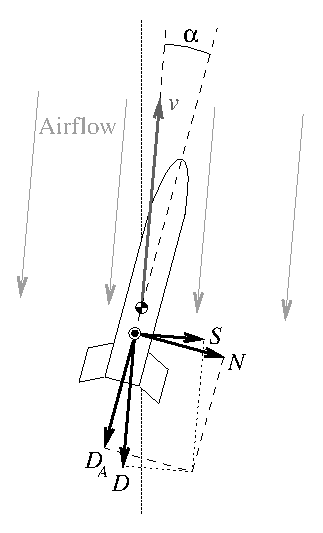
\epsfig{file=figures/aerodynamics/aero-force-components,width=35mm} \\ (b)}
\hfill
\parbox{35mm}{\centering
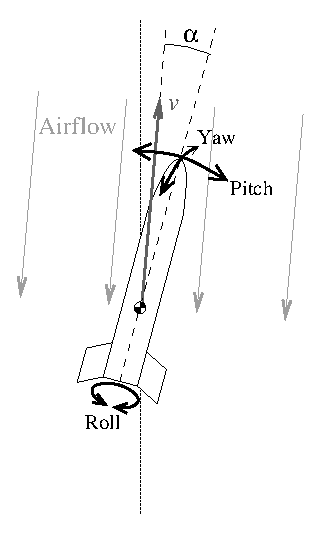
\epsfig{file=figures/aerodynamics/pitch-yaw-roll,width=35mm} \\ (c)}
\caption{(a) Forces acting on a rocket in free flight: gravity $G$,
  motor thrust $T$, drag $D$ and normal force $N$.  (b) Perpendicular
  component pairs of the total aerodynamical force: normal force $N$
  and axial drag $D_A$; side force $S$ and drag $D$.  (c) The pitch,
  yaw and roll directions of a model rocket.}
\label{fig-aerodynamic-forces}
\end{figure}


The three moments around the different axis are called the 
{\it pitch}, {\it yaw} and {\it roll moments}, as depicted in
Figure~\ref{fig-aerodynamic-forces}(c).  Since a typical rocket has no
``natural'' roll angle of flight as an aircraft does, we may choose
the pitch angle to be in the same plane as the angle of attack, \ie
the plane defined by the velocity vector and the centerline of the
rocket.  Thus, the normal force generates the pitching moment and no
other moments.





\subsection{Aerodynamic force coefficients}

When studying rocket configurations, the absolute force values are
often difficult to interpret, since many factors affect them.  In
order to get a value better suited for comparison, the forces are
normalized by the current dynamic pressure $q=\frac{1}{2}\rho v_0^2$
and some characteristic area \Aref\ to get a non-dimensional force
coefficient. Similarly, the moments are normalized by the dynamic
pressure, characteristic area and characteristic length $d$.  Thus,
the normal force coefficient corresponding to the normal force $N$ is
defined as
%
\begin{equation}
C_N  =  \frac{N}{\frac{1}{2}\rho v_0^2 \, \Aref} 
\label{eq-CN-def}
\end{equation}
%
and the pitch moment coefficient for a pitch moment $m$ as
%
\begin{equation}
C_m  =  \frac{m}{\frac{1}{2}\rho v_0^2 \, \Aref\, d}.
\label{eq-Cm-def}
\end{equation}
%
A typical choice of reference area is the base of the rocket's nose
cone and the reference length is its diameter.

The pitch moment is always calculated around some reference point,
while the normal force stays constant regardless of the point of
origin.  If the moment coefficient $C_m$ is known for some reference
point, the moment coefficient at another point $C_m'$ can be
calculated from
%
\begin{equation}
C_m'd = C_md - C_N\Delta x
\label{eq-moment-reference}
\end{equation}
%
where $\Delta x$ is the distance along the rocket centerline.
Therefore it is sufficient to calculate the moment coefficient only at
some constant point along the rocket body.  In this thesis the
reference point is chosen to be the tip of the nose cone.

The {\it center of pressure} (CP) is defined as the position from
which the total normal force alone produces the current pitching
moment.  Therefore the total normal force produces no moment around
the CP itself, and an equation for the location of the CP
can be obtained from (\ref{eq-moment-reference}) by selecting setting
$C_m'=0$:
%
\begin{equation}
X = \frac{C_m}{C_N}\,d
\end{equation}
%
Here $X$ is the position of the CP along the rocket centerline from
the nose cone tip.  This equation is valid when $\alpha>0$.  As
$\alpha$ approaches zero, both $C_m$ and $C_N$ approach zero.  The CP
is then obtained as a continuous extension using l'H�pital's rule
%
\begin{equation}
X = \left.\frac{\;\frac{\partial C_m}{\partial\alpha}\;}
          {\;\frac{\partial C_N}{\partial\alpha}\;}\,d\right|_{\alpha=0}
  = \frac{\Cma}{\CNa}\,d
\label{eq-CP-position}
\end{equation}
%
where the normal force coefficient and pitch moment coefficient
derivatives have been defined as
%
\begin{equation}
\CNa = \left.\frac{\partial C_N}{\partial\alpha}\right|_{\alpha=0}
\hspace{5mm}\mbox{and}\hspace{5mm}
\Cma = \left.\frac{\partial C_m}{\partial\alpha}\right|_{\alpha=0}.
\label{eq-CNa-derivative}
\end{equation}

At very small angles of attack we may approximate $C_N$ and $C_m$ to
be linear with $\alpha$, so to a first approximation
%
\begin{equation}
C_N \approx \CNa\,\alpha
\hspace{5mm}\mbox{and}\hspace{5mm}
C_m \approx \Cma\,\alpha.
\label{eq-CNa-approx}
\end{equation}
%
The Barrowman method uses the coefficient derivatives to determine the
CP position using equation~(\ref{eq-CP-position}).  However, there are
some significant nonlinearities in the variation of $C_N$ as a
function of $\alpha$.  These will be accounted for by holding the
approximation of equation~(\ref{eq-CNa-approx}) exact and letting
\CNa\ and \Cma\ be a function of $\alpha$.  Therefore, for the
purposes of this thesis we define
%
\begin{equation}
\CNa = \frac{C_N}{\alpha}
\hspace{5mm}\mbox{and}\hspace{5mm}
\Cma = \frac{C_m}{\alpha}
\label{eq-CNa-definition}
\end{equation}
%
for $\alpha>0$ and by equation~(\ref{eq-CNa-derivative}) for
$\alpha=0$.  These definitions are compatible, since
equation~(\ref{eq-CNa-definition}) simplifies to the partial
derivative~(\ref{eq-CNa-derivative}) at the limit
$\alpha\rightarrow0$.  This definition also allows us to stay true to
Barrowman's original method which is familiar to many rocketeers.


Similar to the normal force coefficient, the drag coefficient is
defined as
%
\begin{equation}
C_D = \frac{D}{\frac{1}{2}\rho v_0^2 \, \Aref}.
\label{eq-CD-def}
\end{equation}
%
Since the size of the rocket has been factored out, the drag
coefficient at zero angle of attack $C_{D0}$ allows a straightforward
method of comparing the effect of different rocket shapes on drag.
However, this coefficient is not constant and will vary with \eg the
speed of the rocket and its angle of attack.


If each of the fins of a rocket are canted at some angle $\delta>0$
with respect to the rocket centerline, the fins will produce a roll
moment on the rocket.  Contrary to the normal force and pitching
moment, canting the fins will produce a non-zero rolling moment but no
corresponding net force.  Therefore the only quantity computed is the
roll moment coefficient, defined by
%
\begin{equation}
C_l  =  \frac{l}{\frac{1}{2}\rho v_0^2 \, \Aref\, d}
\label{eq-Cl-def}
\end{equation}
%
where $l$ is the roll moment.

It shall be shown later that rockets with axially-symmetrical fin
configurations experience no forces that would produce net yawing
moments. However, a single fin may produce all six types of forces and
moments. The equations for the forces and moments of a single fin will
not be explicitly written out, and they can be computed from the
geometry in question.



\subsection{Velocity regions}

Most of the aerodynamic properties of rockets vary with the velocity
of the rocket.  The important parameter is the {\it Mach number},
which is the free-stream velocity of the rocket divided by the local
speed of sound
%
\begin{equation}
M = \frac{v_0}{c}.
\end{equation}
%
The velocity range encountered by rockets is divided into regions with
different impacts on the aerodynamical properties, listed in
Table~\ref{tab-sonics}.  

In {\it subsonic flight} all of the airflow around the rocket occurs
below the speed of sound.  This is the case for approximately $M<0.8$.
At very low Mach numbers air can be effectively treated as an
incompressible fluid, but already above $M\approx 0.3$ some
compressibility issues may have to be considered.

In {\it transonic flight} some of the air flowing around the rocket
accelerates above the speed of sound, while at other places it remains
subsonic.  Some local shock waves are generated and hard-to-predict
interference effects may occur.  The drag of a rocket has a sharp
increase in the transonic region, making it hard to pass into the
supersonic region.  Transonic flight occurs at Mach numbers of
approximately 0.8--1.2.

In {\it supersonic flight} all of the airflow is faster than the
speed of sound (with the exception of \eg the nose cone tip).  A shock
wave is generated by the nose cone and fins.  In supersonic flight
the drag reduces from that of transonic flight, but is generally
greater than that of subsonic flight.  Above approximately Mach 5 new
phenomena begin to emerge that are not encountered at lower supersonic
speeds. This region is called {\it hypersonic flight}.

\begin{table}
\caption{Velocity regions of rocket flight}
\label{tab-sonics}
\begin{center}
\begin{tabular}{cr@{ -- }l}
Region & \multicolumn{2}{c}{Mach number ($M$)} \\
\hline
Subsonic   & \hspace{10mm} 0   & 0.8 \\
Transonic & 0.8 & 1.2 \\
Supersonic & 1.2 & $\sim5$ \\
Hypersonic & $\sim5$ & \\
\hline
\end{tabular}
\end{center}
\end{table}


Methods for predicting the aerodynamic properties of subsonic flight
and some extensions to supersonic flight will be presented.  Since the
analytical prediction of aerodynamic properties in the transonic
region is quite difficult, this region will be accounted for by using
some suitable interpolation function that corresponds reasonably to
actual measurements. Hypersonic flight will not be considered, since
practically no model or high power rockets ever achieve such speeds.


\subsection{Flow and geometry parameters}

There exist many different parameters that characterize aspects of
flow or a rocket's geometry.  One of the most important flow
parameters is the {\it Reynolds number} $R$.  It is a dimensionless
quantity that characterizes the ratio of inertial forces and viscous
forces of flow.  Many aerodynamic properties depend on the Reynolds
number, defined as
%
\begin{equation}
R = \frac{v_0\; L}{\nu}.
\end{equation}
%
Here $v_0$ is the free-stream velocity of the rocket, $L$ is a
characteristic length and $\nu$ is the kinematic viscosity of air.  It
is notable that the Reynolds number is dependent on a characteristic
length of the object in question. In most cases, the length used is
the length of the rocket.  A typical 30~cm sport model flying at
50~m/s has a corresponding Reynolds number of approximately
1\s000\s000.

Another term that is frequently encountered in aerodynamical equations
has been defined its own parameter $\beta$, which characterizes the
flow speed both in subsonic and supersonic flow:
%
\begin{equation}
\beta = \sqrt{\envert{M^2-1}} =
\left\{
\begin{array}{ll}
\sqrt{1-M^2}, & {\rm if\ } M<1 \\
\sqrt{M^2-1}, & {\rm if\ } M>1
\end{array}
\right.
\end{equation}
%
As the flow speed approaches the transonic region $\beta$ approaches
zero.  This term appears for example in the {\it Prandtl factor} $P$
which corrects subsonic force coefficients for compressible flow:
%
\begin{equation}
P = \frac{1}{\beta} = \frac{1}{\sqrt{1-M^2}}
\label{eq-prandtl-factor}
\end{equation}

It is also often useful to define parameters characterizing general
properties of a rocket.  One such parameter is the {\it caliber},
defined as the maximum body diameter.  The caliber is often used to
indicate relative distances on the body of a rocket, such as the
stability margin.  Another common parameter characterizes the
``slenderness'' of a rocket.  It is the {\it fineness ratio} of a
rocket $f_B$, defined as the length of the rocket body divided by the
maximum body diameter.  Typical model rockets have a fineness ratio in
the range of 10--20, but extreme models may have a fineness ratio as
low as 5 or as large as 50.




\subsection{Coordinate systems}

During calculation of the aerodynamic properties a coordinate system
fixed to the rocket will be used.  The origin of the coordinates is at
the nose cone tip with the positive $x$-axis directed along the rocket
centerline.  This convention is also followed internally in the
produced software.  In the following sections the position of the $y$-
and $z$-axes are arbitrary; the parameter $y$ is used as a general
spanwise coordinate when discussing the fins.  During simulation,
however, the $y$- and $z$-axes are fixed in relation to the rocket,
and do not necessarily align with the plane of the pitching moments.



\clearpage
\section{Normal forces and pitching moments}

Barrowman's method~\cite{barrowman-thesis} for determining the total
normal force coefficient derivative \CNa, the pitch moment
coefficient derivative \Cma\ and the CP location at subsonic speeds
first splits the rocket into simple separate components, then
calculates the CP location and \CNa\ for each component separately and
then combines these to get the desired coefficients and CP
location.  The general assumptions made by the derivation are:
%
\begin{enumerate}
\item The angle of attack is very close to zero.
\item The flow around the body is steady and non-rotational.
\item The rocket is a rigid body.
\item The nose tip is a sharp point.
\item The fins are flat plates.
\item The rocket body is axially symmetric.
\end{enumerate}

The components that will be discussed are nose cones, cylindrical body
tube sections, shoulders, boattails and fins, in an arbitrary
order.  The interference effect between the body and fins will be
taken into account by a separate correction term.  Extensions to
account for body lift and arbitrary fin shapes will also be derived.


\subsection{Axially symmetric body components}

The body of the rocket is assumed to be an axially symmetric body of
rotation.  The entire body could be considered to be a single
component, but in practice it is divided into nose cones, shoulders,
boattails and cylindrical body tube sections.  The geometry of typical
nose cones, shoulders and boattails are described in
Appendix~\ref{app-nosecone-geometry}.

The method presented by Barrowman for calculating the normal force and
pitch moment coefficients at supersonic speeds is based on a
second-order shock expansion method.  However, this assumes that the
body of the rocket is very streamlined, and it cannot handle areas
with a slope larger than than $\sim30^\circ$.  Since the software
allows basically any body shape, applying this method would be
difficult.

Since the emphasis is on subsonic flow, for the purposes of this
thesis the normal force and pitching moments produced by the body are
assumed to be equal at subsonic and supersonic speeds.  The assumption
is that the CP location is primarily affected by the fins.  The effect
of supersonic flight on the drag of the body will be accounted for in
Section~\ref{sec-drag}.



\subsubsection{\CNa\ of body components at subsonic speeds}

The normal force for an axially symmetric body at position $x$ in
subsonic flow is given by
%
\begin{equation}
N(x) = \rho v_0 \; \frac{\partial}{\partial x}[A(x)w(x)]
\label{eq-normal-force}
\end{equation}
%
where $A(x)$ is the cross-sectional area of the body, and the $w(x)$
is the local downwash, given as a function of the angle of attack as
%
\begin{equation}
w(x) = v_0 \sin\alpha.
\end{equation}
%
For angles of attack very close to zero $\sin\alpha\approx\alpha$, but
contrary to the original derivation, we shall not make this
simplification.  From the definition of the normal force
coefficient~(\ref{eq-CN-def}) and equation~(\ref{eq-normal-force}) we
obtain
%
\begin{equation}
C_N(x) = \frac{N(x)}{\frac{1}{2}\rho v_0^2\;\Aref}
       = \frac{2\; \sin\alpha}{\Aref}\; \frac{\dif A(x)}{\dif x}.
\label{eq-CNx}
\end{equation}
%
Assuming that the derivative $\frac{\dif A(x)}{\dif x}$ is
well-defined, we can integrate over the component length $l$ to obtain
%
\begin{equation}
C_N = \frac{2\; \sin\alpha}{\Aref}\;
      \int_0^l \frac{\dif A(x)}{\dif x}\dif x
    = \frac{2\; \sin\alpha}{\Aref}\; [A(l)-A(0)].
\end{equation}
%
We then have
%
\begin{equation}
\CNa = \frac{C_N}{\alpha}
     = \frac{2}{\Aref}\; [A(l)-A(0)]\;
       \underbrace{\frac{\sin\alpha}{\alpha}}_
  {\parbox{10mm}{\scriptsize\centering
  $\rightarrow 1$ as \\ $\alpha\rightarrow0$}}.
\label{eq-body-CNa}
\end{equation}
%
This is the same equation as derived by Barrowman with the exception
of the correction term $\sin\alpha/\alpha$.

Equation~(\ref{eq-body-CNa}) shows that as long as the cross-sectional
area of the component changes smoothly, the normal force coefficient
derivative does not depend on the component shape, only the difference
of the cross-sectional area at the beginning and end.  As a
consequence, according to Barrowman's theory, a cylindrical body tube
has no effect on the normal force coefficient or CP location.
However, the lift due to cylindrical body tube sections has been noted
to be significant for long, slender rockets even at angles of attack
of only a few degrees~\cite{galejs}.  An extension
for the effect of body lift will be given shortly.




\subsubsection{\Cma\ of body components at subsonic speeds}

A normal force $N(x)$ at position $x$ produces a pitching moment
%
\begin{equation}
m(x) = xN(x).
\end{equation}
%
at the nose cone tip.  Therefore the pitching moment coefficient is
%
\begin{equation}
C_m(x) = \frac{m(x)}{\frac{1}{2}\rho v_0^2\;\Aref\, d}
       = \frac{xN(x)}{\frac{1}{2}\rho v_0^2\;\Aref\, d}.
\end{equation}
%
Substituting equation~(\ref{eq-CNx}) we obtain
%
\begin{equation}
C_m(x) = \frac{x\;C_N(x)}{d}
       = \frac{2\; \sin\alpha\; x}{\Aref\, d}\; \frac{\dif A(x)}{\dif x}.
\end{equation}
%
This can be integrated over the length of the body to obtain
%
\begin{equation}
C_m = \frac{2\;\sin\alpha}{\Aref\,d}
        \int_0^l x \left(\od{A(x)}{x}\right) \dif x
    = \frac{2\;\sin\alpha}{\Aref\,d}
        \sbr{ lA(l)-\int_0^l A(x) \dif x }.
\end{equation}
%
The resulting integral is simply the volume of the body $V$.
Therefore we have
%
\begin{equation}
C_m = \frac{2\;\sin\alpha}{\Aref\,d} \sbr{ lA(l)-V }
\end{equation}
%
and
%
\begin{equation}
\Cma = \frac{2}{\Aref\,d}\sbr{ lA(l)-V }\; \frac{\sin\alpha}{\alpha}.
\label{eq-body-Cma}
\end{equation}
%
This is, again, the result derived by Barrowman with the additional
correction term $\sin\alpha/\alpha$.


\subsubsection{Effect of body lift}
\label{sec-body-lift}

The analysis thus far has neglected the effect of body lift as
negligible at small angles of attack.  However, in the flight of long,
slender rockets the lift may be quite significant at angles of attack
of only a few degrees, which may occur at moderate wind
speeds~\cite{galejs}.

Robert Galejs suggested adding a correction term to the body
component \CNa\ to account for body lift~\cite{galejs}.  The normal
force exerted on a cylindrical body at an angle of attack $\alpha$
is~\cite[p.~3-11]{hoerner}
%
\begin{equation}
C_N = K\; \frac{A_{\rm plan}}{\Aref}\; \sin^2\alpha
\end{equation}
%
where $A_{\rm plan} = d\cdot l$ is the planform area of the cylinder
and K is a constant $K\approx 1.1$.  Galejs had simplified the
equation with $\sin^2\alpha\approx\alpha^2$, but this shall not be
performed here.  At small angles of attack, when the approximation is
valid, this yields a linear correction to the value of \CNa.

It is assumed that the lift on non-cylindrical components can be
approximated reasonably well with the same equation.  The CP location
is assumed to be the center of the planform area, that is
%
\begin{equation}
X_{\rm lift} = \frac{\int_0^l x\; 2r(x)\dif x}{A_{\rm plan}}.
\end{equation}
%
This is reminiscent of the CP of a rocket flying at an angle of attack
of $90^\circ$.  For a cylinder the CP location is at the center of the
body, which is also the CP location obtained at the limit with
equation~(\ref{eq-body-CP-position}).  However, for nose cones,
shoulders and boattails it yields a slightly different position than
equation~(\ref{eq-body-CP-position}).

%The value of $K$ has been experimentally fitted to experimental data
%from wind tunnels.






\subsubsection{Center of pressure of body components}

The CP location of the body components can be calculated by
inserting equations~(\ref{eq-body-CNa}) and (\ref{eq-body-Cma}) into
equation~(\ref{eq-CP-position}):
%
\begin{equation}
X_B = \frac{(\Cma)_B}{(\CNa)_B}\;d
    = \frac{lA(l)-V}{A(l)-A(0)}
\label{eq-body-CP-position}
\end{equation}
%
It is worth noting that the correction term $\sin\alpha/\alpha$
cancels out in the division, however, it is still present in the
value of \CNa\ and is therefore significant at large angles of attack.

The whole rocket body could be numerically integrated and the
properties of the whole body computed.  However, it is often more
descriptive to split the body into components and calculate the
parameters separately.  The total CP location can be calculated from
the separate CP locations $X_i$ and normal force coefficient
derivatives $(\CNa)_i$ by the moment sum
%
\begin{equation}
X = \frac{\sum_{i=1}^n X_i(\CNa)_i}{\sum_{i=1}^n (\CNa)_i}.
\label{eq-moment-sum}
\end{equation}
%
In this manner the effect of the separate components can be more
easily analyzed.



\subsection{Planar fins}
\label{sec-planar-fins}

The fins of the rocket are considered separately from the body.  Their
CP location and normal force coefficient are determined and added to
the total moment sum~(\ref{eq-moment-sum}).  The interference between
the fins and the body is taken into account by a separate correction
term.

In addition to the corrective normal force, the fins can induce a roll
rate if each of the fins are canted at an angle $\delta$.  The roll
moment coefficient will be derived separately in
Section~\ref{sec-roll-dynamics}.

Barrowman's original report and thesis derived the equations for
trapezoidal fins, where the tip chord is parallel to the body
(Figure~\ref{fig-fin-geometry}(a)).  The equations can be extended to
\eg elliptical fins~\cite{barrowman-elliptical-fins}
(Figure~\ref{fig-fin-geometry}(b)), but many model rocket fin
designs depart from these basic shapes.  Therefore an
extension is presented that approximates the aerodynamical
properties for a free-form fin defined by a list of $(x,y)$
coordinates (Figure~\ref{fig-fin-geometry}(c)). 


\begin{figure}
\centering
\parbox{35mm}{\centering
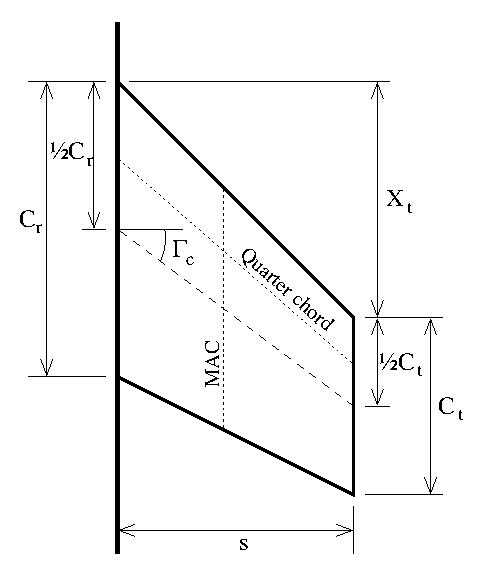
\epsfig{file=figures/fin-geometry/fin-trapezoidal,scale=0.5} \\ (a)}
\hfill
\parbox{35mm}{\centering
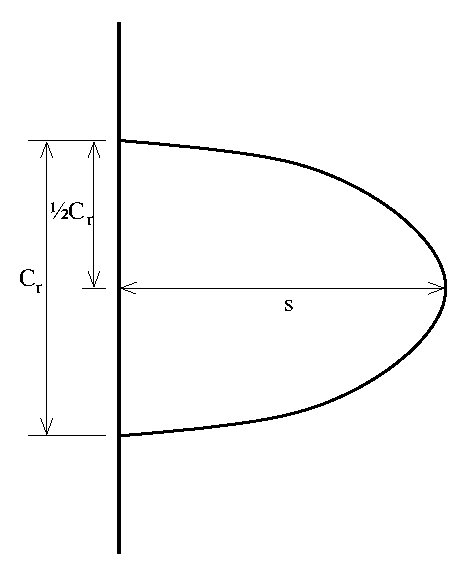
\epsfig{file=figures/fin-geometry/fin-elliptical,scale=0.5} \\ (b)}
\hfill
\parbox{35mm}{\centering
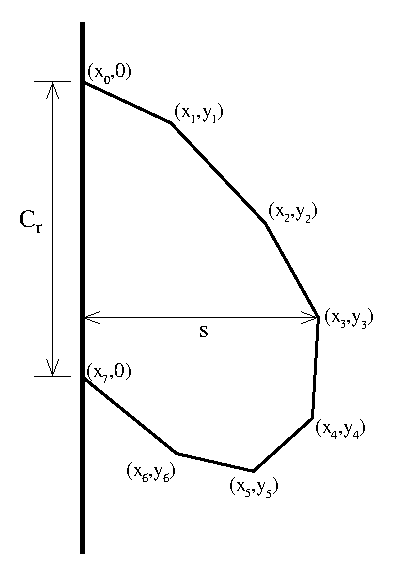
\epsfig{file=figures/fin-geometry/fin-free,scale=0.5} \\ (c)}
\caption{Fin geometry of (a) a trapezoidal fin, (b) an elliptical fin
  and (c) a free-form fin.}
\label{fig-fin-geometry}
\end{figure}



Additionally, Barrowman considered only cases with three or four
fins.  This shall be extended to allow for any reasonable number of
fins, even single fins.


\subsubsection{Center of pressure of fins at subsonic and supersonic
  speeds}

Barrowman argued that since the CP of a fin is located along its mean
aerodynamic chord (MAC) and on the other hand at low subsonic speeds
on its quarter chord, then the CP must be located at the intersection
of these two (depicted in Figure~\ref{fig-fin-geometry}(a)).  He
proceeded to calculate this intersection point analytically from the
fin geometry of a trapezoidal fin.

Instead of following the derivation Barrowman used, an alternative
method will be presented that allows simpler extension to free-form
fins.  The two methods yield identical results for trapezoidal fins.
The length of the MAC $\bar c$, its spanwise position $y_{\rm MAC}$,
and the effective leading edge location $x_{\rm MAC,LE}$ are given
by~\cite{appl-comp-aero-fins}
%
\begin{align}
\bar c &=  \frac{1}{\Afin} \int_0^s c^2(y) \dif y
   \label{eq-MAC-length} \\
y_{\rm MAC} &= \frac{1}{\Afin} \int_0^s yc(y) \dif y 
   \label{eq-MAC-ypos} \\
x_{\rm MAC,LE} &= \frac{1}{\Afin} \int_0^s x_{\rm LE}(y)c(y) \dif y
   \label{eq-MAC-xpos}
\end{align}
%
where $\Afin$ is the one-sided area of a single fin, $s$ is the span of
one fin, and $c(y)$ is the length of the fin chord and $x_{\rm LE}(y)$
the leading edge position at spanwise position $y$.

When these equations are applied to trapezoidal fins and the
lengthwise position of the CP is selected at the quarter chord,
$X_f=x_{\rm MAC,LE}+0.25\,\bar c$,
one recovers exactly the results derived by Barrowman:
%
\begin{align}
y_{\rm MAC} &= \frac{s}{3}\,\frac{C_r+2C_t}{C_r+C_t} \\
X_f &= \frac{X_t}{3}\,\frac{C_r+2C_t}{C_r+C_t} +
          \frac{1}{6}\,\frac{C_r^2+C_t^2+C_rC_t}{C_r+C_t}
\end{align}
%
However, equations~(\ref{eq-MAC-length})--(\ref{eq-MAC-xpos}) may also
be directly applied to elliptical or free-form fins.

Barrowman's method assumes that the lengthwise position of the CP
stays at a constant 25\% of the MAC at subsonic speeds.  However, the
position starts moving rearward above approximately Mach 0.5.  For
$M>2$ the relative lengthwise position of the CP is given by an empirical
formula~\cite[p.~33]{fleeman}
%
\begin{equation}
\frac{X_f}{\bar c} = \frac{\AR\beta - 0.67}{2\AR\beta-1}
\label{eq-fin-CP-mach2}
\end{equation}
%
where $\beta=\sqrt{M^2-1}$ for $M>1$ and \AR\ is the aspect ratio of
the fin defined using the span $s$ as $\AR=2s^2/\Afin$. 
%
Between Mach 0.5 and 2 the lengthwise position of the CP is
interpolated.  A suitable function that gives a curve similar to that
of Figure~2.18 of reference~\cite[p.~33]{fleeman} was found to be a
fifth order polynomial $p(M)$ with the constraints
%
\begin{equation}
  \begin{split}
p(0.5)   & =  0.25 \\
p'(0.5)  & =  0 \\
p(2)     & =  f(2)  \\
p'(2)    & =  f'(2) \\
p''(2)   & =  0 \\
p'''(2)  & =  0
  \end{split}
\end{equation}
%
where $f(M)$ is the function of equation~(\ref{eq-fin-CP-mach2}).



The method presented here can be used to estimate the CP location of
an arbitrary thin fin.  However, problems arise with the method if the
fin shape has a jagged edge as shown in
Figure~\ref{fig-fin-jagged}(a).  If $c(y)$ would include only the sum
of the two separate chords in the area containing the gap, then the
equations would yield the same result as for a fin shown in
Figure~\ref{fig-fin-jagged}(b).  This clearly would be incorrect,
since the position of the latter fin portion would be neglected.  To
overcome this problem, $c(y)$ is chosen as the length from the leading
edge to the trailing edge of the fin, effectively adding the portion
marked by the dotted line to the fin.  This corrects the CP position
slightly rearwards.  The fin area used in
equations~(\ref{eq-MAC-length})--(\ref{eq-MAC-xpos}) must in this case
also be calculated including this extra fin area, but the extra area
must not be included when calculating the normal force coefficient.

This correction is also approximate, since in reality such a jagged
edge would cause some unknown interference factor between the two fin
portions.  Simulating such jagged edges using these methods should
therefore be avoided.


\begin{figure}
\centering
\parbox{35mm}{\centering
\epsfig{file=figures/fin-geometry/fin-jagged,scale=0.5} \\ (a)}
\hspace{5mm}
\parbox{35mm}{\centering
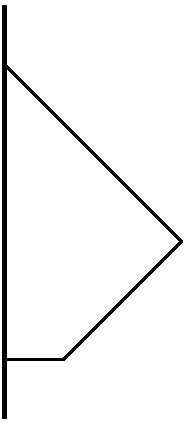
\epsfig{file=figures/fin-geometry/fin-jagged-equivalent,scale=0.5} \\ (b)}
\caption{(a) A jagged fin edge, and (b) an equivalent fin if $c(y)$ is
  chosen to include only the actual fin area.}
\label{fig-fin-jagged}
\end{figure}







\subsubsection{Single fin \CNa\ at subsonic speeds}
\label{sec-average-angle}

Barrowman derived the normal force coefficient derivative value based
on Diederich's semi-empirical method~\cite{diederich}, which states that
for one fin
%
\begin{equation}
\del{\CNa}_1 = \frac{\CNa_0\; F_D \left(\frac{\Afin}{\Aref}\right)
                     \cos\Gamma_c}
             {2+F_D\sqrt{1+\frac{4}{F_D^2}}},
\label{eq-fin-CNa-base}
\end{equation}
%
where
%
\begin{itemize}
\item[$\CNa_0$] = normal force coefficient derivative of a 2D airfoil
\item[$F_D$] = Diederich's planform correlation parameter
\item[$\Afin$] = area of one fin
\item[$\Gamma_c$] = midchord sweep angle (depicted in
  Figure~\ref{fig-fin-geometry}(a)).
\end{itemize}
%
Based on thin airfoil theory of potential flow corrected for
compressible flow
%
\begin{equation}
\CNa_0 = \frac{2\pi}{\beta}
\label{eq-fin-CNa0}
\end{equation}
%
where $\beta=\sqrt{1-M^2}$ for $M<1$.  $F_D$ is a parameter that
corrects the normal force coefficient for the sweep of the fin.
According to Diederich, $F_D$ is given by
%
\begin{equation}
F_D=\frac{\AR}{\frac{1}{2\pi}\CNa_0\cos\Gamma_c}.
\label{eq-fin-FD}
\end{equation}
%
Substituting equations~(\ref{eq-fin-CNa0}), (\ref{eq-fin-FD}) and 
$\AR=2s^2/\Afin$ into (\ref{eq-fin-CNa-base}) and simplifying one
obtains
%
\begin{equation}
%\del{\CNa}_1 = \frac{2\pi\; \AR \del{\frac{\Afin}{\Aref}}}
%             {2+\sqrt{4 + \del{\frac{\beta \AR}{\cos\Gamma_c}}^2}}.
\del{\CNa}_1 = \frac{2\pi\; \frac{s^2}{\Aref}}
             {1+\sqrt{1 + \del{\frac{\beta s^2}{\Afin\cos\Gamma_c}}^2}}.
\label{eq-CNa1}
\end{equation}
%
This is the normal force coefficient derivative for one fin, where the
angle of attack is between the airflow and fin surface.

The value of equation~(\ref{eq-CNa1}) can be calculated directly for
trapezoidal and elliptical fins.  However, in the case of free-form
fins, the question arises of how to define the mid-chord angle
$\Gamma_c$.  If the angle $\Gamma_c$ is taken as the angle from the
middle of the root chord to the tip of the fin, the result may not be
representative of the actual shape, as shown by angle $\Gamma_{c1}$ in
Figure~\ref{fig-midchord-angle}.

\begin{figure}
\centering
\epsfig{file=figures/fin-geometry/fin-midchord-angle,scale=0.7}
\caption{A free-form fin shape and two possibilities for the midchord
  angle $\Gamma_c$.}
\label{fig-midchord-angle}
\end{figure}

Instead the fin planform is divided into a large number of chords, and
the angle between the midpoints of each two consecutive chords is
calculated.  The midchord angle used in equation~(\ref{eq-CNa1}) is
then the average of all these angles.  This produces an angle better
representing the actual shape of the fin, as angle $\Gamma_{c2}$ in
Figure~\ref{fig-midchord-angle}.  The angle calculated by this method
is also equal to the natural midchord angles for trapezoidal and
elliptical fins.




\subsubsection{Single fin \CNa\ at supersonic speeds}
\label{sec-single-fin-CNa-supersonic}

The method for calculating the normal force coefficient of fins at
supersonic speed presented by Barrowman is based on a third-order
expansion according to Busemann theory~\cite{barrowman-fin}.  The
method divides the fin into narrow streamwise strips, the normal force
of which are calculated separately.  In this presentation the method
is further simplified by assuming the fins to be flat plates and by
ignoring a third-order term that corrects for fin-tip Mach cone
effects.

%
% Angle of Inclination = between ray and surface
% Angle of Incidence   = between ray and normal of surface
%


The local pressure coefficient of strip $i$ is calculated by
%
\begin{equation}
C_{P_i} = K_1 \,\eta_i + K_2 \,\eta_i^2 + K_3 \,\eta_i^3
\label{eq-local-pressure-coefficient}
\end{equation}
%
where $\eta_i$ is the inclination of the flow at the surface and the
coefficients are
%
\begin{align}
K_1 &= \frac{2}{\beta} \\
K_2 &= \frac{(\gamma+1)M^4 - 4\,\beta^2}{4\,\beta^4} \\
K_3 &= \frac{(\gamma+1)M^8 + (2\gamma^2-7\gamma-5)M^6 +
  10(\gamma+1)M^4 + 8}{6\,\beta^7}
\end{align}
%
It is noteworthy that the coefficients $K_1$, $K_2$ and $K_3$ can be
pre-calculated for various Mach numbers, which makes the pressure
coefficient of a single strip very fast to compute.  At small
angles of inclination the pressure coefficient is nearly linear, as
presented in Figure~\ref{fig-fin-strip-pressure-coefficient}.


\begin{figure}
\centering
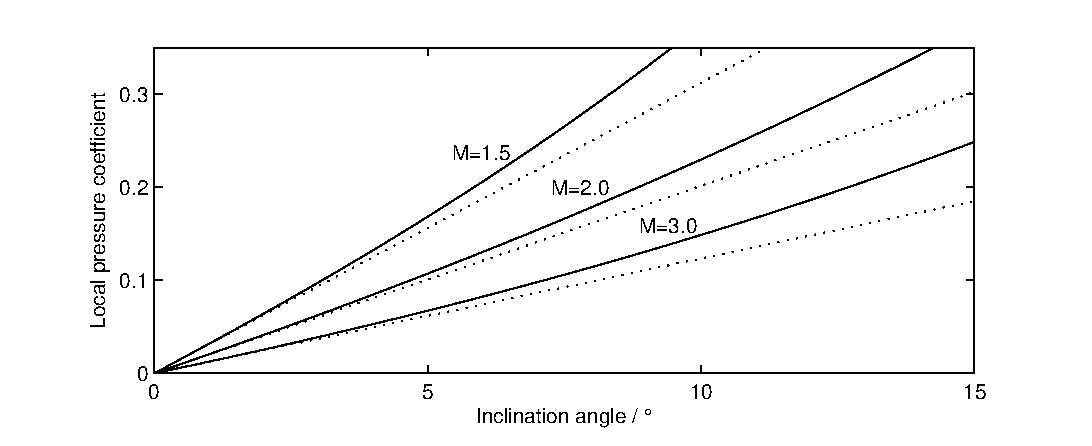
\epsfig{file=figures/fin-geometry/Cp-supersonic,scale=0.6}
\caption{The local pressure coefficient as a function of the
  strip inclination angle at various Mach numbers.  The dotted line
  depicts the linear component of
  equation~(\ref{eq-local-pressure-coefficient}).}
\label{fig-fin-strip-pressure-coefficient}
\end{figure}


%If the rocket is not rolling, the inclinations $\eta_i$ are the
%same for all strips of a fin and only one pressure coefficient needs
%to be computed.  However, presence of a roll velocity generates
%varying inclinations for all strips.  Therefore the current
%examination is performed with separate inclinations and later
%simplified for non-rolling conditions.  The effects of roll are
%further discussed in Section~\ref{sec-roll-dynamics}.

The lift force of strip $i$ is equal to
%
\begin{equation}
F_i = C_{P_i} \cdot \frac{1}{2} \rho v_0^2 \cdot 
  \underbrace{c_i \Delta y}_{\rm area}.
\label{eq-supersonic-strip-lift-force}
\end{equation}
%
The total lift force of the fin is obtained by summing up the
contributions of all fin strips.  The normal force coefficient is then
calculated in the usual manner as
%
\begin{align}
C_N &= \frac{\sum_i F_i}{\frac{1}{2}\rho v_0^2\; \Aref} \\
    &= \frac{1}{\Aref}\sum_i C_{P_i} \cdot c_i\Delta y.
\end{align}

When computing the corrective normal force coefficient of the fins the
effect of roll is not taken into account.  In this case, and
assuming that the fins are flat plates, the inclination angles
$\eta_i$ of all strips are the same, and the pressure coefficient is
constant over the entire fin.  Therefore the normal force coefficient
is simply
%
\begin{equation}
(C_N)_1 = \frac{\Afin}{\Aref} \;C_P.
\end{equation}
%
Since the pressure coefficient is not linear with the angle of attack,
the normal force coefficient slope is defined using
equation~(\ref{eq-CNa-definition}) as
%
\begin{equation}
(\CNa)_1 = \frac{(C_N)_1}{\alpha} = 
 \frac{\Afin}{\Aref} \; \del{K_1 + K_2\,\alpha + K_3\,\alpha^2}.
\end{equation}




\subsubsection{Multiple fin \CNa}
\label{update-roll-angle}

In his thesis, Barrowman considered only configurations with three and
four fins, one of which was parallel to the lateral airflow.  For
simulation purposes, it is necessary to lift these restrictions to
allow for any direction of lateral airflow and for any number of
fins.

The lift force of a fin is perpendicular to the fin and originates
from its CP.  Therefore a single fin may cause a rolling and yawing
moment in addition to a pitching moment.  In this case all of the
forces and moments must be computed from the geometry.  If there are
two or more fins placed symmetrically around the body then the yawing
moments cancel, and if additionally there is no fin cant then the
total rolling moment is also zero, and these moments need not be
computed.

The geometry of an uncanted fin configuration is depicted in
Figure~\ref{fig-dihedral-angle}.  The dihedral angle between each of
the fins and the airflow direction is denoted $\Lambda_i$.  The fin
$i$ encounters a local angle of attack of
%
\begin{equation}
\alpha_i = \alpha \sin\Lambda_i
\end{equation}
%
for which the normal force component (the component parallel to the
lateral airflow) is then
%
\begin{equation}
\del{\CNa}_{\Lambda_i} = \del{\CNa}_1 \sin^2 \Lambda_i.
\end{equation}


\begin{figure}
\centering
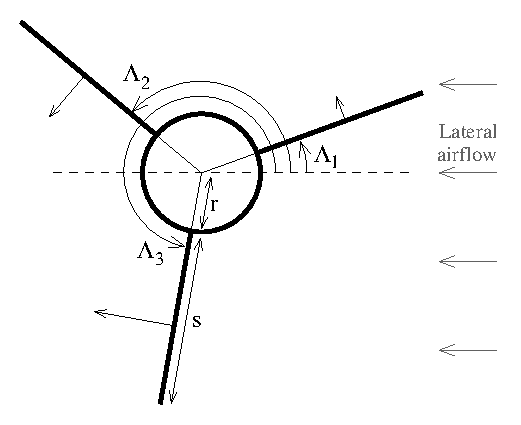
\epsfig{file=figures/fin-geometry/dihedral-angle,scale=1}
\caption{The geometry of an uncanted three-fin configuration (viewed
  from rear).}
\label{fig-dihedral-angle}
\end{figure}


The sum of the coefficients for $N$ fins then yields
%
\begin{equation}
\sum_{k=1}^N \del{\CNa}_{\Lambda_k} =
    \del{\CNa}_1 \sum_{k=1}^N \sin^2\Lambda_k.
\label{N-fin-equation}
\end{equation}
%
However, when $N\geq 3$ and the fins are spaced equally around the
body of the rocket, the sum simplifies to a constant
%
\begin{equation}
\sum_{k=1}^N \sin^2 (2\pi k/N + \theta) = \frac{N}{2}.
\label{N-fin-simplification}
\end{equation}
%
This equation predicts that the normal force produced by three or more
fins is independent of the roll angle $\theta$ of the vehicle.
Investigation by Pettis~\cite{pettis} showed that the normal force
coefficient derivative of a four-finned rocket at Mach~1.48 decreased
by approximately 6\% at a roll angle of $45^\circ$, and the roll angle
had negligible effect on an eight-finned rocket.  Experimental data of
a four-finned sounding rocket at Mach speeds from 0.60 to 1.20
supports the 6\% estimate~\cite{experimental-transonic}.  

The only experimental data available to the author of three-fin
configurations was of a rocket with a rounded triangular body cross
section~\cite{triform-fin-data}.  This data suggests an effect of
approximately 15\% on the normal force coefficient derivative
depending on the roll angle.  However, it is unknown how much of this
effect is due to the triangular body shape and how much from the fin
positioning.

It is also hard to predict such an effect when examining singular
fins.  If three identical or very similar singular fins are placed on
a rocket body, the effect should be the same as when the fins belong
to the same three-fin configuration.  Due to these facts the effect of
the roll angle on the normal force coefficient derivative is ignored
when a fin configuration has three or more fins.
%
\footnote{In OpenRocket versions prior to 0.9.6 a sinusoidal reduction
of 15\% and 6\% was applied to three- and four-fin configurations,
respectively.  However, this sometimes caused a significantly
different predicted CP location compared to the pure Barrowman method,
and also caused a discrepancy when such a fin configuration was
decomposed into singular fins.  It was deemed better to follow the
tested and tried Barrowman method instead of introducing additional
terms to the equation.}

However, in configurations with many fins the fin--fin
interference may cause the normal force to be less than that estimated
directly by equation~(\ref{N-fin-equation}).  According to
reference~\cite[p.~5-24]{MIL-HDBK}, the normal force coefficients
for six and eight-fin configurations are 1.37 and 1.62 times that of
the corresponding four-fin configuration, respectively.  The values
for five and seven-fin configurations are interpolated between these
values.

\pagebreak[4]
Altogether, the normal force coefficient derivative $(\CNa)_N$ is
calculated by:
%
\begin{equation}
(\CNa)_N = \del{\sum_{k=1}^N \sin^2\Lambda_k} \del{\CNa}_1 \cdot
  \left\{ 
\begin{array}{ll}
  1.000\; & N_{\rm tot}=1,2,3,4  \vspace{1mm}\\
  0.948\; & N_{\rm tot}=5  \vspace{1mm}\\
  0.913\; & N_{\rm tot}=6  \vspace{1mm}\\
  0.854\; & N_{\rm tot}=7  \vspace{1mm}\\
  0.810\; & N_{\rm tot}=8  \vspace{1mm}\\
  0.750\; & N_{\rm tot}>8
\end{array}
  \right.
\end{equation}
%
%\begin{equation}
%(\CNa)_N =
%  \left\{ 
%\begin{array}{ll}
%  \del{\sum_{k=1}^N \sin^2\Lambda_k} \del{\CNa}_1 & N=1,2 \vspace{1mm}\\
%  1.50\; \del{\CNa}_1 & N=3  \vspace{1mm}\\
%  2.00\; \del{\CNa}_1 & N=4  \vspace{1mm}\\
%  2.37\; \del{\CNa}_1 & N=5  \vspace{1mm}\\
%  2.74\; \del{\CNa}_1 & N=6  \vspace{1mm}\\
%  2.99\; \del{\CNa}_1 & N=7  \vspace{1mm}\\
%  3.24\; \del{\CNa}_1 & N=8
%\end{array}
%  \right.
%\end{equation}
%
Here $N$ is the number of fins in this fin set, while $N_{\rm tot}$ is
the total number of parallel fins that have an interference effect.
The sum term simplifies to $N/2$ for $N\geq3$ according to
equation~(\ref{N-fin-simplification}).  The interference effect for
$N_{\rm tot}>8$ is assumed at 25\%, as data for such configurations is
not available and such configurations are rare and eccentric in any
case.

\subsubsection{Fin--body interference}

The normal force coefficient must still be corrected for fin--body
interference, which increases the overall produced normal force.  Here
two distinct effects can be identified: the normal force on the fins
due to the presence of the body and the normal force on the body due
to the presence of fins.  Of these the former is significantly larger;
the latter is therefore ignored.  The effect of the extra fin lift is
taken into account using a correction term
%
\begin{equation}
\del{\CNa}_{T(B)} = K_{T(B)}\;\del{\CNa}_N
\end{equation}
%
where $\del{\CNa}_{T(B)}$ is the normal force coefficient derivative
of the tail in the presence of the body.  The term $K_{T(B)}$ can be
approximated by~\cite{barrowman-rd}
%
\begin{equation}
K_{T(B)} = 1 + \frac{r_t}{s + r_t},
\end{equation}
%
where $s$ is the fin span from root to tip and $r_t$ is the body
radius at the fin position.  The value $\del{\CNa}_{T(B)}$ is then
used as the final normal force coefficient derivative of the fins.


%The normal force coefficient must still be corrected for fin--body
%interference, which increases the produced normal force.  The effect
%of the interference can be split into two components, the normal force
%of the fins in the presence of the body $\del{\CNa}_{T(B)}$ and of the
%body in the presence of the fins $\del{\CNa}_{B(T)}$.  (The subscript
%$T$ refers to {\it tail}.)  The interference is taken into account
%using the correction factors
%%
%\begin{align}
%\del{\CNa}_{T(B)} &= K_{T(B)}\;\del{\CNa}_N \\
%\del{\CNa}_{B(T)} &= K_{B(T)}\;\del{\CNa}_N.
%\end{align}
%%
%In his original report, Barrowman simplified the factor $K_{T(B)}$ to
%%
%\begin{equation}
%K_{T(B)} = 1 + \frac{r_t}{s + r_t},
%\end{equation}
%%
%where $s$ is the fin span from root to tip and $r_t$ is the body
%radius at the fin position, and ignored the effect of $K_{B(T)}$ as
%small compared to $K_{T(B)}$ for typical fin dimensions.  However,
%$K_{T(B)}$ may be significant for fins with a span short compared to
%the body radius.  In his thesis, a more accurate equation for
%$K_{T(B)}$ is provided, and $K_{B(T)}$ is given
%as~\cite[p.~31]{barrowman-thesis}
%%
%\begin{equation}
%K_{B(T)} = \del{1 + \frac{r_t}{s + r_t}}^2 - K_{T(B)}.
%\end{equation}
%%
%Therefore the total interference effect can be accounted for by a
%factor
%%
%\begin{equation}
%K_T = K_{T(B)} + K_{B(T)} = \del{1 + \frac{r_t}{s + r_t}}^2
%\end{equation}
%%
%and
%%
%\begin{equation}
%\del{\CNa}_{\rm fins} = K_T\; (\CNa)_N.
%\end{equation}

%This equation takes the increase on body lift and adds it as an
%additional force on the fins.  The equation holds at subsonic speeds
%and also at supersonic speeds until the fin tip Mach cone intersects
%the body.  In the latter case more complex interference factors would
%be required, which have been ignored in the current software.

% TODO: FUTURE: supersonic interference effects, MIL-HDBK page 5-25 or B'man



\pagebreak[4]
\subsection{Pitch damping moment}

So far the effect of the current pitch angular velocity has been
ignored as marginal.  This is the case during the upward flight of a
stable rocket.  However, if a rocket is launched nearly vertically in
still air, the rocket flips over rather rapidly at apogee.  In
some cases it was observed that the rocket was left wildly oscillating
during descent.  The pitch damping moment opposes the fast rotation of
the rocket thus damping the oscillation.

Since the pitch damping moment is notable only at apogee, and
therefore does not contribute to the overall flight characteristics,
only a rough estimate of its magnitude is required.  A cylinder in
perpendicular flow has a drag coefficient of approximately $C_D=1.1$,
with the reference area being the planform area of the
cylinder~\cite[p.~3-11]{hoerner}.  Therefore a short piece of cylinder
$\dif\xi$ at a distance $\xi$ from a rotation axis, as shown in
Figure~\ref{fig-pitch-velocity}, produces a force
%
\begin{equation}
\dif F = 1.1 \cdot \frac{1}{2}\rho(\omega\xi)^2 \cdot 
\underbrace{2r_t\,\dif\xi}_{\rm ref.area}
\end{equation}
%
when the cylinder is rotating at an angular velocity $\omega$.  The
produced moment is correspondingly $\dif m = \xi\dif F$.  Integrating
this over $0\ldots l$ yields the total pitch moment
%
\begin{equation}
m = 0.275 \cdot \rho\, r_t\, l^4 \omega^2
\end{equation}
%
and thus the moment damping coefficient is
%
\begin{equation}
C_{\rm damp} = 
    0.55 \cdot \frac{l^4\; r_t}{\Aref\, d}\cdot\frac{\omega^2}{v_0^2}.
\end{equation}
%
This value is computed separately for the portions of the rocket body
fore and aft of the CG using an average body radius as $r_t$.

\begin{figure}
\centering
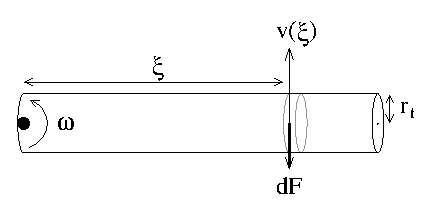
\epsfig{file=figures/components/body-pitch-rate,scale=0.8}
\caption{Pitch damping moment due to a pitching body component.}
\label{fig-pitch-velocity}
\end{figure}



Similarly, a fin with area $\Afin$ at a distance $\xi$ from the CG
produces a moment of approximately
%
\begin{equation}
C_{\rm damp} = 
    0.6\cdot \frac{N\,\Afin\;\xi^3}{\Aref\,d}\cdot\frac{\omega^2}{v_0^2}
\end{equation}
%
where the effective area of the fins is assumed to be 
$\Afin\cdot N/2$.  For $N>4$ the value $N=4$ is used, since the other
fins are not exposed to any direct airflow.

The damping moments are applied to the total pitch moment in the
opposite direction of the current pitch rate.  It is noteworthy
that the damping moment coefficients are proportional to $\omega^2/v_0^2$,
confirming that the damping moments are insignificant during most of
the rocket flight, where the angles of deflection are small and the
velocity of the rocket large.  Through roll coupling the yaw rate may also
momentarily become significant, and therefore the same correction is
also applied to the yaw moment.





\clearpage
\section{Roll dynamics}
\label{sec-roll-dynamics}

When the fins of a rocket are canted at some angle $\delta>0$, the
fins induce a rolling moment on the rocket.  On the other hand, when a
rocket has a specific roll velocity, the portions of the fin far from
the rocket centerline encounter notable tangential velocities
which oppose the roll.  Therefore a steady-state roll velocity,
dependent on the current velocity of the rocket, will result.

The effect of roll on a fin can be examined by dividing the fin into
narrow streamwise strips and later integrating over the strips.  A
strip $i$ at distance $\xi_i$ from the rocket centerline encounters a
radial velocity
%
\begin{equation}
u_i = \omega \xi_i
\end{equation}
%
where $\omega$ is the angular roll velocity, as shown in
Figure~\ref{fig-roll-velocity}.  The radial velocity induces an angle
of attack
%
\begin{equation}
\eta_i = \tan^{-1} \del{\frac{u_i}{v_0}} =
\tan^{-1}\del{\frac{\omega\xi_i}{v_0}}
\approx \frac{\omega\xi_i}{v_0}
\label{eq-tan-approx}
\end{equation}
%
to the strip.  The approximation $\tan^{-1} \eta \approx \eta$ is
valid for $u_i\ll v_0$, that is, when the velocity of the rocket is
large compared to the radial velocity.  The approximation is
reasonable up to angles of $\eta \approx 20^\circ$, above which angle
most fins stall, which limits the validity of the equation in any
case.  

When a fin is canted at an angle $\delta$, the total
inclination of the strip to the airflow is
%
\begin{equation}
\alpha_i = \delta - \eta_i.
\label{eq-roll-aoa-variation}
\end{equation}

Assuming that the force produced by a strip is directly proportional
to the local angle of attack, the force on strip $i$ is
%
\begin{equation}
F_i = k_i \alpha_i = k_i (\delta - \eta_i)
\end{equation}
%
for some $k_i$.  The total moment produced by the fin is then
%
\begin{equation}
%l = \int_0^s (r+y) k (\delta-\eta(y))\dif y
%  = \int_0^s (r+y) k \delta \dif y - \int_0^s (r+y) k \eta(y) \dif y
l = \sum_i \xi_i F_i = \sum_i \xi_i k_i (\delta - \eta_i)
  = \sum_i \xi_i k_i \delta - \sum_i \xi_i k_i \eta_i.
\end{equation}
%
This shows that the effect of roll can be split into two components:
the first term $\sum_i \xi_i k_i \delta$ is the roll moment induced by
a fin canted at the angle $\delta$ when flying at zero roll rate
($\omega=0$), while the second term $\sum_i \xi_i k_i \eta_i$ is the
opposing moment generated by an uncanted fin ($\delta=0$) when flying
at a roll rate $\omega$.  These two moments are called the roll
forcing moment and roll damping moment, respectively.  These
components will be analyzed separately.


\begin{figure}
\centering
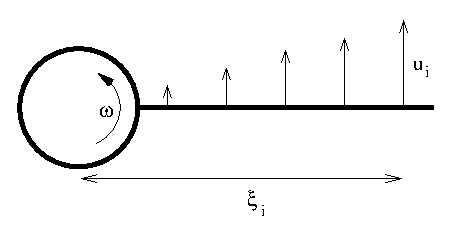
\epsfig{file=figures/fin-geometry/roll-velocity,scale=0.8}
\caption{Radial velocity at different positions of a fin.  Viewed from
  the rear of the rocket.}
\label{fig-roll-velocity}
\end{figure}



\subsection{Roll forcing coefficient}

As shown previously, the roll forcing coefficient can be computed by
examining a rocket with fins canted at an angle $\delta$ flying at
zero roll rate ($\omega=0$).  In this case, the cant angle $\delta$ acts
simply as an angle of attack for each of the fins.  Therefore, the
methods computed in the previous section can be directly applied.
Because the lift force of a fin originates from the mean aerodynamic
chord, the roll forcing coefficient of $N$ fins is equal to
%
\begin{equation}
C_{lf} = \frac{N (y_{\rm MAC}+r_t) \del{\CNa}_1 \delta}{d}
\label{eq-roll-forcing-moment}
\end{equation}
%
where $y_{\rm MAC}$ and $\del{\CNa}_1$ are computed using the methods
described in Section~\ref{sec-planar-fins} and $r_t$ is the radius of
the body tube at the fin position.  This result is applicable
for both subsonic and supersonic speeds.



\subsection{Roll damping coefficient}

The roll damping coefficient is computed by examining a rocket with
uncanted fins ($\delta=0$) flying at a roll rate $\omega$.  Since
different portions of the fin encounter different local angles of
attack, the damping moment must be computed from the separate
streamwise airfoil strips.

At subsonic speeds the force generated by strip $i$ is equal to
%
\begin{equation}
F_i = \CNa_0 \; \frac{1}{2}\rho v_0^2 \; 
\underbrace{c_i \Delta\xi_i}_{\rm area} \; \eta_i.
\end{equation}
%
Here $\CNa_0$ is calculated by equation~(\ref{eq-fin-CNa0}) and 
$c_i \Delta\xi_i$ is the area of the strip.  The roll damping moment
generated by the strip is then
%
\begin{equation}
\del{C_{ld}}_i
  = \frac{F_i\,\xi_i}{\frac{1}{2}\rho v_0^2\,\Aref\, d}
  = \frac{\CNa_0}{\Aref\,d} \; \xi_i c_i\Delta\xi_i \; \eta_i.
\end{equation}
%
By applying the approximation~(\ref{eq-tan-approx}) and summing
(integrating) the airfoil strips the total roll damping moment for $N$
fins is obtained as:
%
\begin{align}
C_{ld} & = N \sum_i (C_{ld})_i \nonumber \\
& = \frac{N \;\CNa_0\;\omega}{\Aref\,d\,v_0} \sum_i c_i\xi_i^2\Delta\xi_i.
\label{eq-roll-damping-moment}
\end{align}
%
The sum term is a constant for a specific fin shape.  It can be
computed numerically from the strips or analytically for specific
shapes.  For trapezoidal fins the term can be integrated as
%
\begin{equation}
\sum_i c_i\xi_i^2\Delta\xi_i = 
\frac{C_r+C_t}{2}\;r_t^2s + \frac{C_r+2C_t}{3}\;r_ts^2 + 
\frac{C_r+3C_t}{12}\;s^3
\end{equation}
%
and for elliptical fins
%
\begin{equation}
\sum_i c_i\xi_i^2\Delta\xi_i = 
C_r \del{ \frac{\pi}{4}\;r_t^2s + \frac{2}{3}\;r_ts^2 +
  \frac{\pi}{16}\;s^3 }.
\end{equation}


The roll damping moment at supersonic speeds is calculated
analogously, starting from the supersonic strip lift force,
equation~(\ref{eq-supersonic-strip-lift-force}), where the angle of
inclination of each strip is calculated using
equation~(\ref{eq-tan-approx}).  The roll moment at supersonic speeds
is thus
%
\begin{equation}
C_{ld} = \frac{N}{\Aref\,d} \sum_i C_{P_i}\, c_i \xi_i \Delta \xi_i.
\end{equation}
%
The dependence on the incidence angle $\eta_i$ is embedded within the
local pressure coefficient $C_{P_i}$,
equation~(\ref{eq-local-pressure-coefficient}).  Since the dependence
is non-linear, the sum term is a function of the Mach number as well
as the fin shape.




\subsection{Equilibrium roll frequency}

One quantity of interest when examining rockets with canted fins
is the steady-state roll frequency that the fins induce on a rocket
flying at a specific velocity.  This is obtained by equating the roll
forcing moment~(\ref{eq-roll-forcing-moment}) and roll damping
moment~(\ref{eq-roll-damping-moment}) and solving for the roll rate
$\omega$.  The equilibrium roll frequency at subsonic speeds is
therefore
%
\begin{equation}
f_{\rm eq} = \frac{\omega_{\rm eq}}{2\pi} =
\frac{\Aref\; \beta v_0 \; y_{\rm MAC} \; (\CNa)_1 \; \delta}
{4\pi^2\; \sum_i c_i\xi_i^2\Delta\xi_i}
\label{eq-subsonic-roll-rate}
\end{equation}
%
It is worth noting that the arbitrary reference area \Aref\ is
cancelled out by the reference area appearing within $(\CNa)_1$,
as is to be expected.

At supersonic speeds the dependence on the incidence angle is
non-linear and therefore the equilibrium roll frequency must be solved
numerically.  Alternatively, the second and third-order terms of the
local pressure coefficient of
equation~(\ref{eq-local-pressure-coefficient}) may be ignored, in
which case an approximation for the equilibrium roll frequency nearly
identical to the subsonic case is obtained:
%
\begin{equation}
f_{\rm eq} = \frac{\omega_{\rm eq}}{2\pi} =
\frac{\Aref\; \beta v_0 \; y_{\rm MAC} \; (\CNa)_1 \; \delta}
{4\pi\; \sum_i c_i\xi_i^2\Delta\xi_i}
\label{eq-supersonic-roll-rate}
\end{equation}
%
The value of $(\CNa)_1$ must, of course, be computed using different
methods in the subsonic and supersonic cases.




%\subsection{Roll sensitivity}
%
%The vast majority of model rockets have uncanted fins and in
%principle no roll is induced to these rockets.  However, in practice
%imprecision in the attachment of the fins and other protrusions always
%cause some roll to the rocket during flight.  In some applications,
%such as launching rockets with onboard video cameras, it is desirable
%to design the rockets so as to minimize the roll rate.  To assist this
%design, a quantity called the {\it roll sensitivity} of the rocket is
%defined as
%%
%\begin{equation}
%f_{\rm sens} = \frac{1}{N}\eval{\pd{f_{\rm eq}}{\delta}}_{\delta=0}.
%\end{equation}
%%
%This is the slope of the equilibrium roll frequency at $\delta=0$,
%divided by the number of fins.  If measured in units of 
%$\rm Hz/^\circ$, the quantity indicates the number of rotations per
%second induced by one fin being attached at an angle of $1^\circ$.  By
%minimizing the roll sensitivity of a rocket, the effect of
%construction imperfections on the roll rate can be minimized.  From
%equation~(\ref{eq-roll-rate}) the subsonic roll sensitivity is
%obtained as
%%
%\begin{equation}
%f_{\rm sens} =
%\frac{\Aref\; \beta v_0 \; y_{\rm MAC} \; (\CNa)_1}
%{N\; 4\pi^2\; \sum_i c_i\xi_i^2\Delta\xi_i}
%\end{equation}
%%
%or conversely,
%%
%\begin{equation}
%f_{\rm eq} = N\; f_{\rm sens}\,\delta.
%\end{equation}
%%
%Similarly, in supersonic flight the roll sensitivity may either be
%solved numerically, or computed using the linear approximation for
%$C_{P_i}$ yielding 
%%
%\begin{equation}
%f_{\rm sens} = 
%\frac{\Aref\; \beta v_0 \; y_{\rm MAC} \; (\CNa)_1}
%{N\; 4\pi\; \sum_i c_i\xi_i^2\Delta\xi_i}.
%\end{equation}
%
%
%When the fins are canted by design, the roll sensitivity loses its
%significance.  Therefore if all the fins on a rocket are uncanted, the
%quantity of intrest is the roll sensitivity, while for a rocket with
%canted fins it is the equilibrium roll frequency.






\clearpage
\section{Drag forces}
\label{sec-drag}

Air flowing around a solid body causes drag, which resists the
movement of the object relative to the air.  Drag forces arise from
two basic mechanisms, the air pressure distribution around the rocket
and skin friction.  The pressure distribution is further divided into
body pressure drag (including shock waves generated as supersonic
speeds), parasitic pressure drag due to protrusions such as launch
lugs and base drag.  Additional sources of drag include interference
between the fins and body and vortices generated at fin tips when
flying at an angle of attack.  The different drag sources are depicted
in Figure~\ref{fig-drag-components}.  Each drag source will be analyzed
separately; the interference drag and fin-tip vortices will be
ignored as small compared to the other sources.

As described in Section~\ref{sec-general-aerodynamics}, two different
drag coefficients can be defined: the (total) drag coefficient $C_D$
and the axial drag coefficient $C_A$.  At zero angle of attack these
two coincide, $C_{D_0} = C_{A_0}$, but at other angles a distinction
between the two must be made.  The value of significance in the
simulation is the axial drag coefficient $C_A$ based on the choice of
force components.  However, the drag coefficient $C_D$ describes the
deceleration force on the rocket, and is a more commonly known value
in the rocketry community, so it is informational to calculate its
value as well.

In this section the zero angle-of-attack drag coefficient
$C_{D_0} = C_{A_0}$ will be computed first.  Then, in
Section~\ref{sec-axial-drag} this will be extended for angles of
attack and $C_A$ and $C_D$ will be computed.  Since the drag force of
each component is proportional to its particular size, the subscript
$\bullet$ will be used for coefficients that are computed using the
reference area of the specific component.  This reference area is the
frontal area of the component unless otherwise noted.  Conversion to
the global reference area is performed by
%
\begin{equation}
C_{D_0} = \frac{A_{\rm component}}{\Aref} \cdot C_{D\bullet}.
\end{equation}


\begin{figure}
\centering
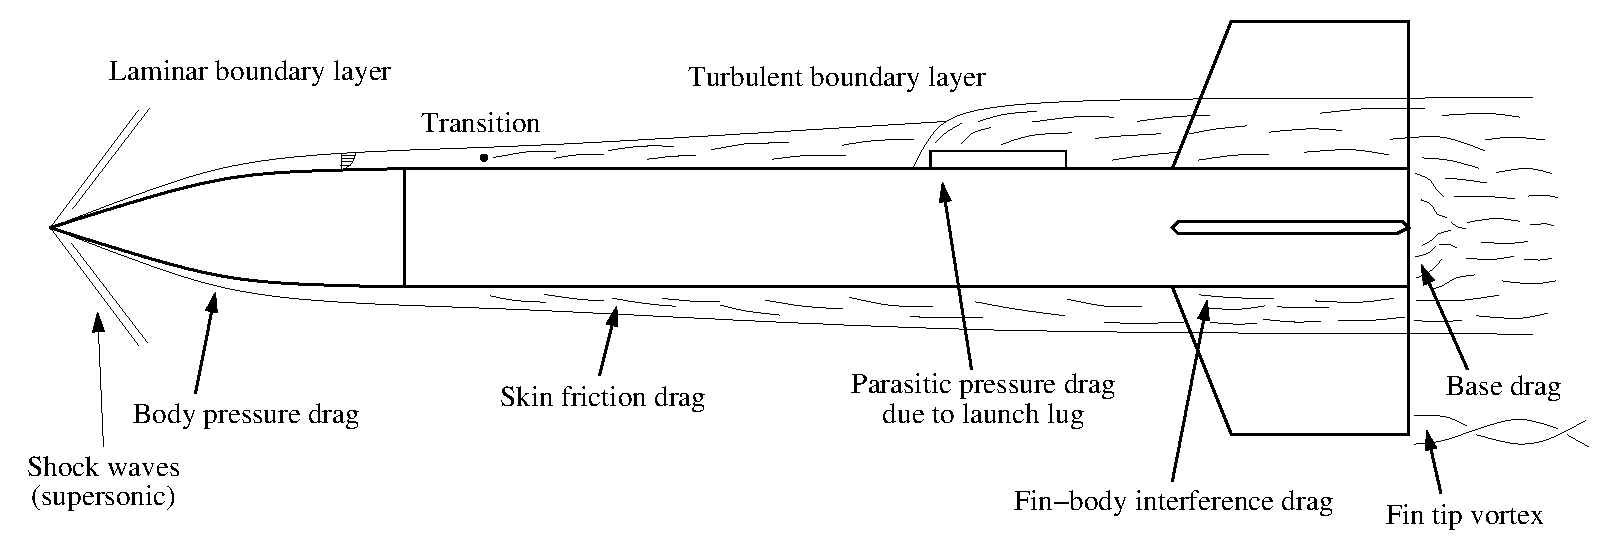
\epsfig{file=figures/aerodynamics/drag-components,width=13.5cm}
\caption{Types of model rocket drag at subsonic speeds.}
\label{fig-drag-components}
\end{figure}


\subsection{Laminar and turbulent boundary layers}

At the front of a streamlined body, air flows smoothly around the
body in layers, each of which has a different velocity.  The layer
closest to the surface ``sticks'' to the object having zero velocity.
Each layer gradually increases the speed until the free-stream
velocity is reached.  This type of flow is said to be {\it laminar}
and to have a {\it laminar boundary layer}.  The thickness of the
boundary layer increases with the distance the air has flowed along
the surface.  At some point a transition occurs and the layers of air
begin to mix.  The boundary layer becomes {\it turbulent} and thickens
rapidly.  This transition is depicted in
Figure~\ref{fig-drag-components}.

A turbulent boundary layer induces a notably larger skin friction drag
than a laminar boundary layer.  It is therefore necessary to consider
how large a portion of a rocket is in laminar flow and at what point
the flow becomes turbulent.  The point at which the flow becomes
turbulent is the point that has a {\it local critical Reynolds number}
%
\begin{equation}
R_{\rm crit} = \frac{v_0 \; x}{\nu},
\label{eq-transition-Re}
\end{equation}
%
where $v_0$ is the free-stream air velocity, $x$ is the distance along
the body from the nose cone tip and 
$\nu\approx 1.5\cdot10^{-5}\;\rm m^2/s$ is the kinematic viscosity of
air.  The critical Reynolds number is approximately 
$R_{\rm crit} = 5\cdot10^5$~\cite[p.~43]{barrowman-thesis}. Therefore,
at a velocity of 100~m/s the transition therefore occurs approximately
7~cm from the nose cone tip.

% Air viscosity:
% http://www.engineeringtoolbox.com/air-absolute-kinematic-viscosity-d_601.html


%Since the drag force is approximately proportional to the square of
%the free-stream velocity, the value of $C_D$ is most critical at high
%velocities.  Equation~(\ref{eq-transition-Re}) shows that at a velocity
%of 100~m/s the transition to turbulent flow occurs about 7~cm
%from the nose cone tip.  Therefore at these speeds most of the wetted
%area of a typical model rocket is in turbulent flow.

Surface roughness or even slight protrusions may also trigger the
transition to occur prematurely.  At a velocity of 60~m/s the critical
height for a cylindrical protrusion all around the body is of the
order of 0.05~mm~\cite[p.~348]{advanced-model-rocketry}.  The
body-to-nosecone joint, a severed paintbrush hair or some other
imperfection on the surface may easily exceed this limit and cause
premature transition to occur.

Barrowman presents methods for computing the drag of both fully
turbulent boundary layers as well as partially-laminar layers.  Both
methods were implemented and tested, but the difference in apogee
altitude was less than 5\% in with all tested designs.  Therefore,
the boundary layer is assumed to be fully turbulent in all cases.

%A typical model rocket may therefore be assumed to have a fully
%turbulent boundary layer.  Only sport models which have been
%finished to fine precision may benefit from a partial laminar
%flow around the rocket.  These different types of rockets will be
%taken into account by having two modes of calculation, one for typical
%model rockets that assumes a fully turbulent boundary layer, and
%another one which assumes very fine precision finish.






\subsection{Skin friction drag}

Skin friction is one of the most notable sources of model rocket
drag.  It is caused by the friction of the viscous flow of air
around the rocket.  In his thesis Barrowman presented formulae for
estimating the skin friction coefficient for both laminar and
turbulent boundary layers as well as the transition between the
two~\cite[pp.~43--47]{barrowman-thesis}.  As discussed above, a fully
turbulent boundary layer will be assumed in this thesis.

The skin friction coefficient $C_f$ is defined as the drag coefficient
due to friction with the reference area being the total wetted area
of the rocket, that is, the body and fin area in contact with the
airflow:
%
\begin{equation}
C_f = \frac{D_{\rm friction}}{\frac{1}{2} \rho v_0^2\;A_{\rm wet}}
\end{equation}
%
The coefficient is a function of the rocket's Reynolds number $R$ and
the surface roughness.  The aim is to first calculate the skin
friction coefficient, then apply corrections due to compressibility
and geometry effects, and finally to convert the coefficient to the
proper reference area.


\subsubsection{Skin friction coefficients}
\label{sec-skin-friction-coefficient}

The values for $C_f$ are given by different formulae depending on the
Reynolds number.  For fully turbulent flow the coefficient is given by
%
\begin{equation}
C_f = \frac{1}{(1.50\; \ln R - 5.6)^2}.
\label{eq-turbulent-friction}
\end{equation}

The above formula assumes that the surface is ``smooth'' and the
surface roughness is completely submerged in a thin, laminar sublayer.
At sufficient speeds even slight roughness may have an effect on the
skin friction.  The critical Reynolds number corresponding to the
roughness is given by
%
\begin{equation}
R_{\rm crit} = 51\left(\frac{R_s}{L}\right)^{-1.039},
\end{equation}
%
where $R_s$ is an approximate roughness height of the surface.  A few
typical roughness heights are presented in Table~\ref{tab-roughnesses}.
For Reynolds numbers above the critical value, the skin friction
coefficient can be considered independent of Reynolds number, and has
a value of
%
\begin{equation}
C_f = 0.032\left(\frac{R_s}{L}\right)^{0.2}.
\label{eq-critical-friction}
\end{equation}
%


\begin{table}
\caption{Approximate roughness heights of different
  surfaces~\cite[p.~5-3]{hoerner}}
\label{tab-roughnesses}
\begin{center}
\begin{tabular}{lc}
Type of surface & Height / \um \\
\hline
Average glass                  & 0.1 \\
Finished and polished surface  & 0.5 \\
Optimum paint-sprayed surface  & 5 \\
Planed wooden boards           & 15 \\
% planed = h�yl�tty ???
Paint in aircraft mass production & 20 \\
Smooth cement surface          & 50 \\
Dip-galvanized metal surface   & 150 \\
Incorrectly sprayed aircraft paint & 200 \\
Raw wooden boards              & 500 \\
Average concrete surface       & 1000 \\
\hline
\end{tabular}
\end{center}
\end{table}


Finally, a correction must be made for very low Reynolds numbers.  The
experimental formulae are applicable above approximately
$R\approx10^4$.  This corresponds to velocities typically below 1~m/s,
which therefore have negligible effect on simulations.  Below this
Reynolds number, the skin friction coefficient is assumed to be equal
as for $R=10^4$.

Altogether, the skin friction coefficient for turbulent flow is
calculated by
%
\begin{equation}
C_f = \left\{
\begin{array}{ll}
1.48\cdot10^{-2}, & \mbox{if $R<10^4$} \\
\mbox{Eq.~(\ref{eq-turbulent-friction})}, & \mbox{if $10^4<R<R_{\rm crit}$} \\
\mbox{Eq.~(\ref{eq-critical-friction})}, & \mbox{if $R>R_{\rm crit}$}
\end{array}
\right. .
\end{equation}
%
These formulae are plotted with a few different surface roughnesses in
Figure~\ref{fig-skinfriction-plot}.  Included also is the laminar and
transitional skin friction values for comparison.

\begin{figure}
\centering
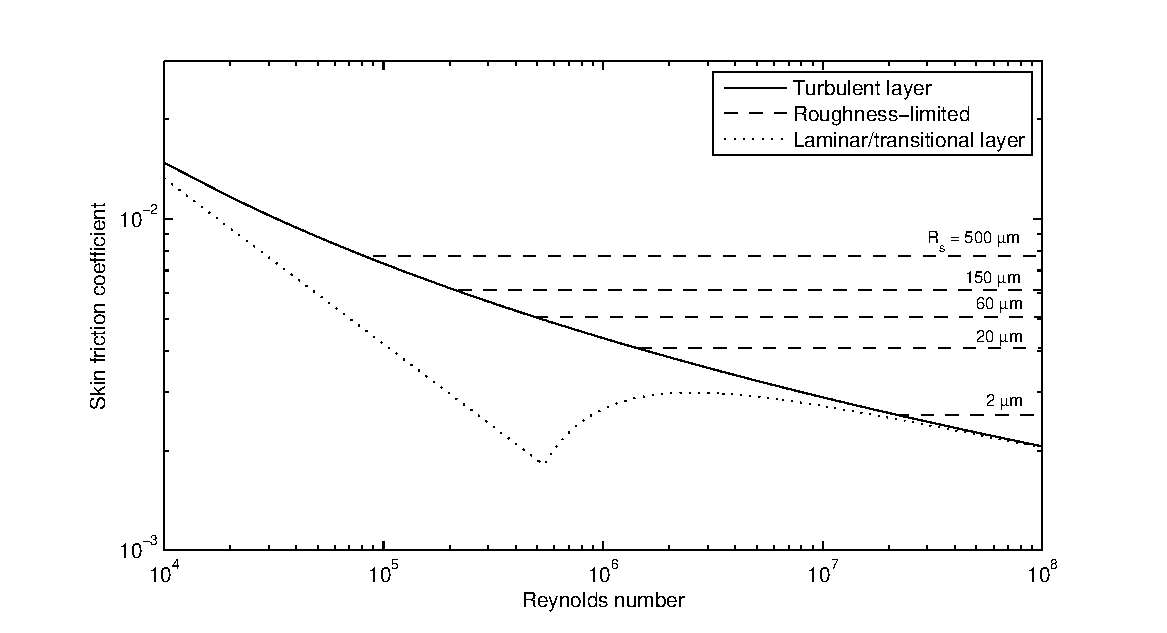
\epsfig{file=figures/drag/skin-friction-coefficient,width=11cm}
\caption{Skin friction coefficient of turbulent, laminar and
  roughness-limited boundary layers.}
\label{fig-skinfriction-plot}
\end{figure}


\subsubsection{Compressibility corrections}

A subsonic speeds the skin friction coefficient turbulent and
roughness-limited boundary layers need to be corrected for
compressibility with the factor
%
\begin{equation}
{C_f}_c = C_f\; (1-0.1\, M^2).
\end{equation}
%
In supersonic flow, the turbulent skin friction coefficient must be
corrected with
%
\begin{equation}
{C_f}_c = \frac{C_f}{(1+0.15\, M^2)^{0.58}}
\end{equation}
%
and the roughness-limited value with
%
\begin{equation}
{C_f}_c = \frac{C_f}{1 + 0.18\, M^2}.
\end{equation}
%
However, the corrected roughness-limited value should not be used if
it would yield a value smaller than the corresponding turbulent
value.


\subsubsection{Skin friction drag coefficient}
\label{sec-skin-friction-drag}

After correcting the skin friction coefficient for compressibility
effects, the coefficient can be converted into the actual drag
coefficient.  This is performed by scaling it to the correct reference
area.  The body wetted area is corrected for its cylindrical geometry,
and the fins for their finite thickness.
%effect of finite fin thickness which Barrowman handled
%separately is also included~\cite[p.~55]{barrowman-thesis}.  
The total friction drag coefficient is then
%
\begin{equation}
(C_D)_{\rm friction} = {C_f}_c \; \frac{
  \del{1 + \frac{1}{2f_B}} \cdot A_{\rm wet,body} + 
  \del{1 + \frac{2t}{\bar c}} \cdot A_{\rm wet,fins}}
   {\Aref}
\label{eq-friction-drag-scale}
\end{equation}
%
where $f_B$ is the fineness ratio of the rocket, and $t$ the thickness
and $\bar c$ the mean aerodynamic chord length of the fins.  The
wetted area of the fins $A_{\rm wet,fins}$ includes both sides of the
fins.





\subsection{Body pressure drag}

Pressure drag is caused by the air being forced around the rocket.  A
special case of pressure drag are shock waves generated at supersonic
speeds.  In this section methods for estimating the pressure drag of
nose cones will be presented and reasonable estimates also for
shoulders and boattails.


\subsubsection{Nose cone pressure drag}

At subsonic speeds the pressure drag of streamlined nose cones is
significantly smaller than the skin friction drag.  In fact, suitable
shapes may even yield negative pressure drag coefficients, producing a
slight reduction in drag.  Figure~\ref{fig-nosecone-cd} presents
various nose cone shapes and their respective measured pressure drag
coefficients.~\cite[p.~3-12]{hoerner}

It is notable that even a slight rounding at the joint between the nose
cone and body reduces the drag coefficient dramatically.  Rounding the
edges of an otherwise flat head reduces the drag coefficient from 0.8
to 0.2, while a spherical nose cone has a coefficient of only 0.01.
The only cases where an appreciable pressure drag is present is when
the joint between the nose cone and body is not smooth, which may
cause slight flow separation.

The nose pressure drag is approximately
proportional to the square of the sine of the joint angle $\phi$
(shown in
Figure~\ref{fig-nosecone-cd})~\cite[p.~237]{handbook-supersonic-aerodynamics}:
%
\begin{equation}
(C_{D\bullet,M=0})_p = 0.8 \cdot \sin^2\phi.
\label{eq-nosecone-pressure-drag}
\end{equation}
%
This yields a zero pressure drag for all nose cone shapes that have a
smooth transition to the body.  The equation does not take into
account the effect of extremely blunt nose cones (length less than
half of the diameter).  Since the main drag cause is slight flow
separation, the coefficient cannot be corrected for compressibility
effects using the Prandtl coefficient, and the value is applicable
only at low subsonic velocities.

\begin{figure}
\centering
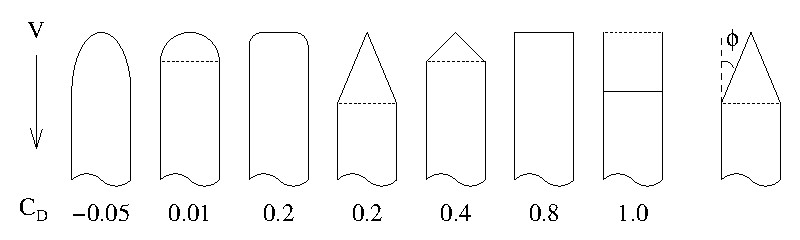
\epsfig{file=figures/nose-geometry/nosecone-cd-top,width=11cm}
\caption{Pressure drag of various nose cone
  shapes~\cite[p.~3-12]{hoerner}.}
\label{fig-nosecone-cd}
\end{figure}


At supersonic velocities shock waves increase the pressure drag
dramatically. In his report Barrowman uses a second-order
shock-expansion method that allows determining the pressure
distribution along an arbitrary slender rotationally symmetrical
body~\cite{second-order-shock-expansion-method}.  However,
the method has some problematic limitations.  The method cannot handle
body areas that have a slope larger than approximately $30^\circ$,
present in several typical nose cone shapes.  The local airflow in
such areas may decrease below the speed of sound, and the method
cannot handle transonic effects.  Drag in the transonic
region is of special interest for rocketeers wishing to build rockets
capable of penetrating the sound barrier.

Instead of a general piecewise computation of the air pressure around
the nose cone, a simpler semi-empirical method for estimating the
transonic and supersonic pressure drag of nose cones is used.  The
method, described in detail in
Appendix~\ref{app-nosecone-drag-method}, combines theoretical and
empirical data of different nose cone shapes to allow estimating the
pressure drag of all the nose cone shapes described in
Appendix~\ref{app-nosecone-geometry}.

The semi-empirical method is used at Mach numbers above 0.8.  
At high subsonic velocities the pressure drag is interpolated between
that predicted by equation~(\ref{eq-nosecone-pressure-drag}) and the
transonic method.  The pressure drag is assumed to be non-decreasing
in the subsonic region and to have zero derivative at $M=0$.  A
suitable interpolation function that resembles the shape of the
Prandtl factor is
%
\begin{equation}
(C_{D\bullet})_{\rm pressure} = a\cdot M^b + (C_{D\bullet,M=0})_p
\label{eq-nosecone-pressure-interpolator}
\end{equation}
%
where $a$ and $b$ are computed to fit the drag coefficient and its
derivative at the lower bound of the transonic method.



\subsubsection{Shoulder pressure drag}

Neither Barrowman nor Hoerner present theoretical or experimental
data on the pressure drag of transitions at subsonic velocities.  In
the case of shoulders, the pressure drag coefficient is assumed to be
the same as that of a nose cone, except that the reference area is the
difference between the aft and fore ends of the transition.  The
effect of a non-smooth transition at the beginning of the shoulder is
ignored, since this causes an increase in pressure and thus cannot
cause flow separation.

While this assumption is reasonable at subsonic velocities, it is
somewhat dubious at supersonic velocities.  However, no comprehensive
data set of shoulder pressure drag at supersonic velocities was
found.  Therefore the same assumption is made for supersonic
velocities and a warning is generated during such simulations (see
Section~\ref{sec-warnings}).  The refinement of the supersonic
shoulder pressure drag estimation is left as a future enhancement.



\subsubsection{Boattail pressure drag}

The estimate for boattail pressure drag is based on the body base
drag estimate, which will be presented in Section~\ref{sec-base-drag}.
At one extreme, the transition length is zero, in which case the
boattail pressure drag will be equal to the total base drag.  On the
other hand, a gentle slope will allow a gradual pressure change
causing approximately zero pressure drag.  Hoerner has presented
pressure drag data for wedges, which suggests that at a
length-to-height ratio below 1 has a constant pressure drag
corresponding to the base drag and above a ratio of 3 the pressure
drag is negligible.  Based on this and the base drag
equation~(\ref{eq-base-drag}), an approximation for the pressure drag
of a boattail is given as
%
\begin{equation}
(C_{D\bullet})_{\rm pressure} =
\frac{A_{\rm base}}{A_{\rm boattail}} \cdot (C_{D\bullet})_{\rm base}
\cdot 
\left\{
\begin{array}{cl}
1 & \mbox{if\ } \gamma < 1 \\
\frac{3-\gamma}{2} & \mbox{if\ } 1 < \gamma < 3 \\
0 & \mbox{if\ } \gamma > 3
\end{array}
\right.
\end{equation}
%
where the length-to-height ratio $\gamma = l/(d_1-d_2)$ is calculated
from the length and fore and aft diameters of the boattail.  The
ratios 1 and 3 correspond to reduction angles of $27^\circ$ and
$9^\circ$, respectively, for a conical boattail.  The base drag
$(C_{D\bullet})_{\rm base}$ is calculated using
equation~(\ref{eq-base-drag}).

Again, this approximation is made primarily based on subsonic data.
At supersonic velocities expansion fans exist, the counterpart of
shock waves in expanding flow.  However, the same equation is used for
subsonic and supersonic flow and a warning is generated during
transonic simulation of boattails.



\subsection{Fin pressure drag}

The fin pressure drag is highly dependent on the fin profile shape.
Three typical shapes are considered, a rectangular profile, rounded
leading and trailing edges, and an airfoil shape with rounded leading
edge and tapering trailing edge.  Barrowman estimates the fin pressure
drag by dividing the drag further into components of a finite
thickness leading edge, thick trailing edge and overall fin
thickness~\cite[p.~48--57]{barrowman-thesis}.  In this report the fin
thickness was already taken into account as a correction to the skin
friction drag in Section~\ref{sec-skin-friction-drag}.  The division
to leading and trailing edges also allows simple extension to the
different profile shapes.

The drag of a rounded leading edge can be considered as a circular
cylinder in cross flow with no base drag.  Barrowman derived 
an empirical formula for the leading edge pressure drag as
%
\begin{equation}
(C_{D\bullet})_{LE\perp} = 
\left\{ 
\begin{array}{ll}
  (1-M^2)^{-0.417} - 1 & \mbox{for $M<0.9$} \\
  1-1.785(M-0.9)         & \mbox{for $0.9 < M < 1$} \\
  1.214 - \frac{0.502}{M^2} + \frac{0.1095}{M^4} & \mbox{for $M>1$}
\end{array}
  \right. .
\end{equation}
%
The subscript $\perp$ signifies the the flow is perpendicular to the
leading edge.

In the case of a rectangular fin profile the leading edge pressure
drag is equal to the stagnation pressure drag as derived in 
equation~\ref{eq-blunt-cylinder-drag} of
Appendix~\ref{app-blunt-cylinder-drag}:
\begin{equation}
(C_{D\bullet})_{LE\perp} = (C_{D\bullet})_{\rm stag}
\end{equation}

The leading edge pressure drag of a slanted fin is obtained from the
cross-flow principle~\cite[p.~3-11]{hoerner} as
%
\begin{equation}
(C_{D\bullet})_{LE} = (C_{D\bullet})_{LE\perp} \cdot \cos^2\Gamma_L
\end{equation}
%
where $\Gamma_L$ is the leading edge angle.  Note that in the equation
both coefficients are relative to the frontal area of the cylinder, so
the ratio of their reference areas is also $\cos\Gamma_L$.  In the
case of a free-form fin the angle $\Gamma_L$ is the average leading
edge angle, as described in Section~\ref{sec-average-angle}.

The fin base drag coefficient of a square profile fin is the same as
the body base drag coefficient in equation~\ref{eq-base-drag}:
%
\begin{equation}
(C_{D\bullet})_{TE} = (C_{D\bullet})_{\rm base}
\end{equation}
%
For fins with rounded edges the value is taken as half of the total
base drag, and for fins with tapering trailing edges the base
drag is assumed to be zero.

The total fin pressure drag is the sum of the leading and trailing
edge drags
%
\begin{equation}
(C_{D\bullet})_{\rm pressure} = 
(C_{D\bullet})_{LE} + (C_{D\bullet})_{TE}.
\end{equation}
%
The reference area is the fin frontal area $N\cdot ts$.

% TODO: FUTURE: supersonic shock wave drag???





\subsection{Base drag}
\label{sec-base-drag}

Base drag is caused by a low-pressure area created at the base of the
rocket or in any place where the body radius diminishes rapidly
enough.  The magnitude of the base drag can be estimated using the
empirical formula~\cite[p.~23]{fleeman}
%
\begin{equation}
(C_{D\bullet})_{\rm base} = 
  \left\{ 
\begin{array}{ll}
  0.12+0.13M^2, & \mbox{if $M<1$} \\
  0.25/M,         & \mbox{if $M>1$}
\end{array}
  \right. .
\label{eq-base-drag}
\end{equation}
%
The base drag is disrupted when a motor exhausts into the area.  A
full examination of the process would need much more detailed
information about the motor and would be unnecessarily complicated.  A
reasonable approximation is achieved by subtracting the area of the
thrusting motors from the base reference area~\cite[p.~23]{fleeman}.
Thus, if the base is the same size as the motor itself, no base drag
is generated.  On the other hand, if the base is large with only a
small motor in the center, the base drag is approximately the same as
when coasting.

The equation presented above ignores the effect that the rear body
slope angle has on the base pressure.  A boattail at the end of the
rocket both diminishes the reference area of base drag, thus reducing
drag, but the slope also directs air better into the low pressure
area. This effect has been neglected as small compared to the effect
of reduced base area.









\subsection{Parasitic drag}

Parasitic drag refers to drag caused by imperfections and protrusions
on the rocket body.  The most significant source of parasitic drag in
model rockets are the launch guides that protrude from the rocket
body.  The most common type of launch guide is one or two launch lugs,
which are pieces of tube that hold the rocket on the launch rod during
takeoff.  Alternatives to launch lugs include replacing the tube with
metal wire loops or attaching rail pins that hold the rocket on a
launch rail.  These three guide types are depicted in
Figure~\ref{fig-launch-guides}.  The effect of launch lugs on the
total drag of a model rocket is small, typically in the range of
0--10\%, due to their comparatively small size.  However, studying
this effect may be of notable interest for model rocket designers.


\begin{figure}
\centering
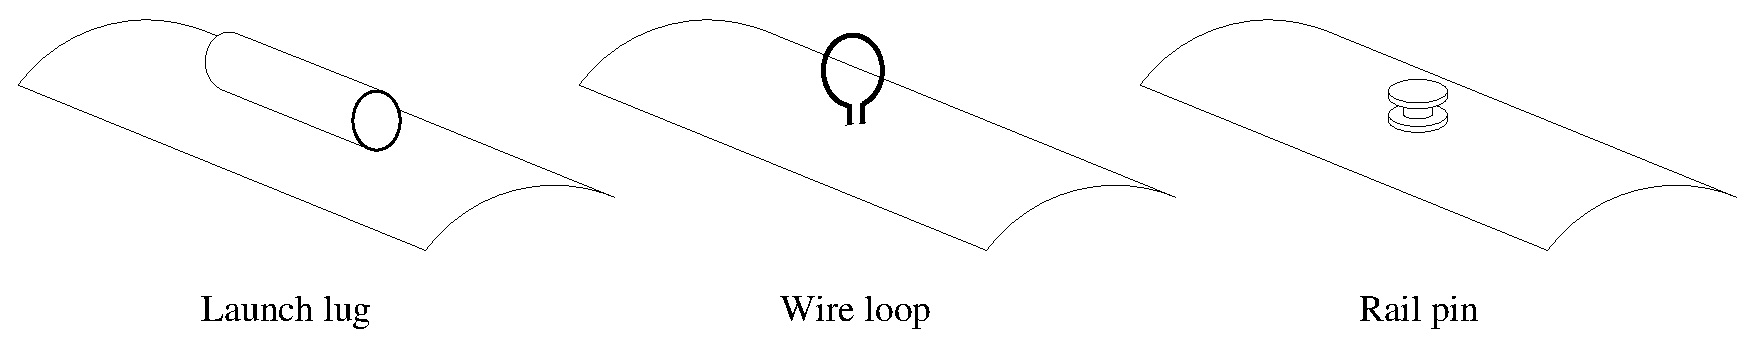
\epsfig{file=figures/components/launch-guides,width=12cm}
\caption{Three types of common launch guides.}
\label{fig-launch-guides}
\end{figure}


A launch lug that is long enough that no appreciable airflow occurs
through the lug may be considered a solid cylinder next to the main
rocket body.  A rectangular protrusion that has a length at least
twice its height has a drag coefficient of 0.74, with reference area
being its frontal area~\cite[p.~5-8]{hoerner}.  The drag coefficient
varies proportional to the stagnation pressure as in the case of a
blunt cylinder in free airflow, presented in
Appendix~\ref{app-blunt-cylinder-drag}.

A wire held perpendicular to airflow has instead a drag coefficient of
1.1, where the reference area is the planform area of the
wire~\cite[p.~3-11]{hoerner}.  A wire loop may be thought of as a
launch lug with length and wall thickness equal to the thickness of
the wire.  However, in this view of a launch lug the reference area
must not include the inside of the tube, since air is free to flow
within the loop.

These two cases may be unified by changing the used reference area as
a function of the length of the tube $l$.  At the limit $l=0$ the
reference area is the simple planform area of the loop, and when the
length is greater than the diameter $l>d$ the reference area includes
the inside of the tube as well.  The slightly larger drag coefficient
of the wire may be taken into account as a multiplier to the blunt
cylinder drag coefficient.

Therefore the drag coefficient of a launch guide can be approximately
calculated by
%
\begin{equation}
(C_{D\bullet})_{\rm parasitic} = 
\max\{1.3-0.3\;l/d, 1\} \cdot (C_{D\bullet})_{\rm stag}
\end{equation}
%
where $(C_{D\bullet})_{\rm stag}$ is the stagnation pressure
coefficient calculated in equation~(\ref{eq-blunt-cylinder-drag}), and
the reference area is
%
\begin{equation}
A_{\rm parasitic} = \pi r_{ext}^2 - \pi r_{int}^2 \cdot
\max\{1-l/d,0\}.
\end{equation}

This approximation may also be used to estimate the drag of rail
pins.  A circular pin protruding from a wall has a drag coefficient of
0.80~\cite[p.~5-8]{hoerner}.  Therefore the drag of the pin is
approximately equal to that of a lug with the same frontal area.  The
rail pins can be approximated in a natural manner as launch lugs with
the same frontal area as the pin and a length equal to their
diameter.




\subsection{Axial drag coefficient}
\label{sec-axial-drag}

The total drag coefficient may be calculated by simply scaling the
coefficients to a common reference area and adding them together:
%
\begin{equation}
C_{D_0} = \sum_T \frac{A_T}{\Aref}(C_{D\bullet})_T
 + (C_D)_{\rm friction}
\end{equation}
%
where the sum includes the pressure, base and parasitic drags.  The
friction drag was scaled to the reference area \Aref\ already in
equation~(\ref{eq-friction-drag-scale}).

This yields the total drag coefficient at zero angle of attack.  At an
angle of attack the several phenomena begin to affect the drag.
More frontal area is visible to the airflow, the pressure gradients
along the body change and fin-tip vortices emerge.  On the other hand,
the drag force is no longer axial, so the axial drag force is less
than the total drag force.

Based on experimental data an empirical formula was produced for
calculating the axial drag coefficient at an angle of attach $\alpha$
from the zero-angle drag coefficient.  The scaling function is a
two-part polynomial function that starts from 1 at $\alpha=0^\circ$,
increases to 1.3 at $\alpha=17^\circ$ and then decreases to zero at
$\alpha=90^\circ$; the derivative is also zero at these points.  Since
the majority of the simulated flight is at very small angles of
attack, this approximation provides a sufficiently accurate estimate
for the purposes of this thesis.


\section{Tumbling bodies}
\label{sec-tumbling-bodies}

% Renaming of test vs. models here:
%
% #1  ->  test 2
% #2  ->  test 3
% #3  ->  test 5
% #4  ->  test 4
% #5  ->  test 6
%
% Test 1 failed to produce a reliable result.  Dimensions:
% n=3, Cr=50, Ct=25, s=50, l0=10, d=18, l=74, m=8.1

In staged rockets the lower stages of the rocket separate from the
main rocket body and descend to the ground on their own.  While large
rockets typically have parachutes also in lower stages, most model
rockets rely on the stages falling to the ground without any recovery
device.  As the lower stages normally are not aerodynamically stable,
they tumble during descent, significantly reducing their speed.

This kind of tumbling is difficult if not impossible to model in
6-DOF, and the orientation is not of interest anyway.
For simulating the descent of aerodynamically unstable stages, it is
therefore sufficient to compute the average aerodynamic drag of
the tumbling lower stage.

While model rockets are built in very peculiar forms, staged rockets
are typically much more conservative in their design.  The lower
stages are most often formed of just a body tube and fins.  Five such
models were constructed for testing their descent aerodynamic drag.

Models \#1 and \#2 are identical except for the number of fins.  \#3
represents a large, high-power booster stage.  \#4 is a body tube
without fins, and \#5 fins without a body tube.

\begin{table}
\caption{Physical properties and drop results of the lower stage models}
\label{tab-lower-stages}
\begin{center}
\parbox{80mm}{
\begin{tabular}{cccccc}
Model       & \#1 & \#2 & \#3 & \#4 & \#5 \\
\hline
No. fins    & 3   & 4   & 3   & 0   & 4    \\
$C_r$ / mm  & 70  & 70  & 200 & -   & 85   \\
$C_t$ / mm  & 40  & 40  & 140 & -   & 85   \\
$s$ / mm    & 60  & 60  & 130 & -   & 50   \\
$l_0$ / mm  & 10  & 10  & 25  & -   & -    \\
$d$ / mm    & 44  & 44  & 103 & 44  & 0    \\
$l$ / mm    & 108 & 108 & 290 & 100 & -    \\
$m$ / g     & 18.0& 22.0& 160 & 6.8 & 11.5 \\
\hline
$v_0$ / m/s & 5.6 & 6.3 & 6.6 & 5.4 & 5.0  \\
\end{tabular}
}
\parbox{50mm}{
\epsfig{file=figures/lower-stage/lower-stage,width=50mm}
}
\end{center}
\end{table}

The models were dropped from a height of 22 meters and the drop
was recorded on video.  From the video frames the position of
the component was determined and the terminal velocity $v_0$
calculated with an accuracy of approximately $\pm 0.3\;\rm m/s$.
During the drop test the temperature was -5$^\circ$C, relative
humidity was 80\% and the dew point -7$^\circ$C.  Together these yield
an air density of $\rho = 1.31\rm\;kg/m^3$.  The physical properties
of the models and their terminal descent velocities are listed in
Table~\ref{tab-lower-stages}.

For a tumbling rocket, it is reasonable to assume that the drag force
is relative to the profile area of the rocket.  For body tubes the
profile area is straightforward to calculate.  For three and four fin
configurations the minimum profile area is taken instead.

Based on the results of models \#4 and \#5 it is clear that the
aerodynamic drag coefficient (relative to the profile area) is
significantly different for the body tube and fins.  Thus we assume
the drag to consist of two independent components, one for the fins
and one for the body tube.

At terminal velocity the drag force is equal to that of gravity:
%
\begin{equation}
\frac{1}{2}\rho v_0^2\; (C_{D,f}A_f  + C_{D,bt}A_{bt}) = mg
\end{equation}
%
The values for $C_{D,f}$ and $C_{D,bt}$ were varied to optimize the
relative mean square error of the $v_0$ prediction, yielding a result
of $C_{D,f} = 1.42$ and $C_{D,bt} = 0.56$.  Using these values, the
predicted terminal velocities varied between $3\%\ldots14\%$ from the
measured values.

During optimization it was noted that changing the error function
being optimized had a significant effect on the resulting fin drag
coefficient, but very little on the body tube drag coefficient.  It is
assumed that the fin tumbling model has greater inaccuracy in this
aspect.

It is noteworthy that the body tube drag coefficient 0.56 is exactly
half of that of a circular cylinder perpendicular to the
airflow~\cite[p.~3-11]{hoerner}. This is expected of a cylinder that
is falling at a random angle of attack.  The fin drag coefficient 1.42
is also similar to that of a flat plate 1.17 or an open hemispherical
cup 1.42 \cite[p.~3-17]{hoerner}.

The total drag coefficient $C_D$ of a tumbling lower stage is obtained
by combining and scaling the two drag coefficient components:
%
\begin{equation}
C_D = \frac{C_{D,f}A_f  + C_{D,bt}A_{bt}}{\Aref}
\end{equation}
%
Here $A_{bt}$ is the profile area of the body, and $A_f$ the effective
fin profile area, which is the area of a single fin multiplied by the
efficiency factor.  The estimated efficiency factors for various
numbers of fins are listed in Table~\ref{tab-lower-stage-fins}.

\begin{table}
\caption{Estimated fin efficiency factors for tumblig lower stages}
\label{tab-lower-stage-fins}
\begin{center}
\begin{tabular}{cc}
Number  & Efficiency \\
of fins & factor     \\
\hline
1 & 0.50 \\
2 & 1.00 \\
3 & 1.50 \\
4 & 1.41 \\
5 & 1.81 \\
6 & 1.73 \\
7 & 1.90 \\
8 & 1.85 \\
\hline
\end{tabular}
\end{center}
\end{table}

